%%%%%%%%%%%%%%%%%%%%%%%%%%%%%%%%%%%%%%%%%%%%%%%%%%%%%%%%%%%%%%%%%%%%%%
% Documento PRINCIPAL da newsletter da Comissão de
% Pedometria da Sociedade Brasileira de Ciência do Solo
%
% NÃO EDITE ESSE ARQUIVO!
% 
% Language: Latex
% 
%%%%%%%%%%%%%%%%%%%%%%%%%%%%%%%%%%%%%%%%%%%%%%%%%%%%%%%%%%%%%%%%%%%%%%


% PREÂMBULO
\documentclass[a4paper]{report}

% Língua e codificação
\usepackage[brazilian]{babel}
\usepackage[utf8]{inputenc}
\usepackage[T1]{fontenc}

% para boot
\usepackage{amssymb,amsmath}

% Nota: é preciso incluir o pacote amsmath antes do pacote PEDOMETRIAnews
% porque o último redefine o ambiente de equações...
\usepackage{PEDOMETRIAnews}
\usepackage[round]{natbib}

% Figuras
\usepackage{graphicx}
\usepackage{wrapfig}

% para Sweave
\usepackage{listings}
\usepackage{Sweave}

% cor para verbatim
\usepackage{color}
\let\oldv\verbatim
\let\oldendv\endverbatim
\def\verbatim{\par\setbox0\vbox\bgroup\oldv}
\def\endverbatim{\oldendv\egroup\fboxsep0pt \noindent\colorbox[gray]{0.8}{\usebox0}\par}

% para tcltk-update
\usepackage{shortvrb}
%\usepackage{chapterbib}

\sloppy{}

% links
\usepackage[pdftex]{hyperref} % Deve ser o último pacote carregado
\hypersetup{colorlinks=true, citecolor=blue, linkcolor=blue, urlcolor=blue}

% DOCUMENTO
\begin{document}
 
% Edição da newsletter
\volume{2}
\volnumber{2}
\date{Jun-Set 2013}
\titlepage

\begin{article}
   \title{Editorial}
\author{por Alessandro Samuel-Rosa}
\maketitle
\begin{wrapfigure}{l}{0.15\textwidth}
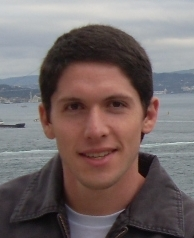
\includegraphics[width=0.15\textwidth]{figuras/foto-alessandro}
\end{wrapfigure}
O segundo número da \textit{Newsletter} da Comissão de Pedometria está cheio de novidades. A principal delas é a nova estrutura, muito mais bonita, graças à inestimável colaboração da comissão editorial do GRASS News, a newsletter do projeto \href{http://grass.osgeo.org/newsletter/}{GRASS}. Após contato com Martin Wegmann \email{wegmann@biozentrum.uni-wuerzburg.de}, editor-chefe do GRASS News, e Dylan Beaudette \email{debeaudette@ucdavis.edu}, administrador da página da web do GRASS News, formos gentilmente autorizados a usar o arquivo de estilo \texttt{GRASSnews.sty}, originalmente derivado do arquivo de estilo \texttt{Rnews.sty}, usado pela equipe do projeto \R{} para produção da sua newsletter. O agora arquivo de estilo da \textit{Newsletter} da Comissão de Pedometria da SBCS, \texttt{PEDOMETRIAnews.sty}, está disponível para baixar \href{http://goo.gl/OBWF3s}{clicando aqui}. É por meio do arquivo de estilo \texttt{PEDOMETRIAnews.sty} que a \textit{Newsletter} fica com a cara que ela tem hoje. Mais informações sobre o uso de \LaTeX{} para a produção de documentos técnico-científicos podem ser encontradas no site da \href{http://www.elsevier.com/author-schemas/preparing-documents-with-tex}{Elsevier}.\\
A evolução da \textit{Newsletter} em seu segundo número acompanha a evolução da pedometria no Brasil, claramente evidenciada pelo volume de trabalhos publicados no Congresso Brasileiro de Ciência do Solo (CBCS), em Florianópolis, há alguns meses atrás. Somam-se aí os espaços destinados mesas de discussão constituídas por importantes pesquisadores da pedometria nacional e internacional. O espaço destinado pela Comissão Organizadora do CBCS mostra que a comunidade científica nacional, assim como já ocorre há mais de uma década em outros países, está muito interessada nas contribuições da mais nova disciplina da ciência do solo. Uma disciplina que exige, como mostram os artigos que seguem, uma abordagem mais do que multidisciplinar ou interdisciplinar. Uma disciplina que exige uma abordagem \href{http://www.fisica-interessante.com/files/artigo-transdisciplinaridade.pdf}{transdisciplinar}, forçando-nos a transpor os limites das disciplinas tradicionais da ciência do solo e mergulhar em um universo de novas maneiras de 
encarar velhos problemas.
%%% Local Variables: 
%%% mode: latex
%%% TeX-master: documento-principal.tex
%%% End: 


\end{article}

\begin{article}
   \title{Mapeamento de solos no nosso tempo}
\author{por Marcos Bacis Ceddia}
\maketitle
\section{Apresentação}
\begin{wrapfigure}{l}{0.15\textwidth}
 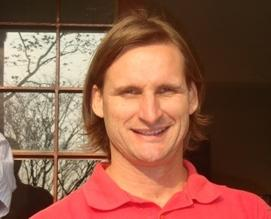
\includegraphics[width=0.15\textwidth]{figuras/bacis}
\end{wrapfigure}
Nos últimos anos, em função do desenvolvimento e disponibilização de tecnologias digitais, a área de mapeamento de solos vem passando por um processo intenso de transformação. A transformação em curso é muito abrangente, implicando em mudanças não somente dos procedimentos técnicos de mapeamento de solos (atividades de escritório, campo e laboratório), mas também de como a informação de solos é transmitida para a sociedade (ensino e extensão). Obviamente, dada a abrangência da transformação, é natural que surjam grandes incertezas, e também oportunidades. Para que instituições e procedimentos mudem, as pessoas precisam mudar. A mudança a que me refiro não é o de negação ao passado e sim de seu completo entendimento, valorização e correta conexão com o nosso tempo e também com o futuro. Precisamos disso para dar continuidade a uma rica história de mapeamento e de conhecimento dos solos de nosso território. Por isso, o título desse texto é o ``Mapeamento de Solos no Nosso Tempo''.
\section{Contexto e objetivos}
Esse texto se baseia amplamente na palestra por mim apresentada no XXXIV Congresso Brasileiro de Ciência do Solo intitulada \emph{``Interfaces entre o Mapeamento Convencional e Digital de Solos''}, a qual ocorreu em julho de 2013 no município de Florianópolis. A palestra foi apresentada no simpósio 17 sobre Pedometria: Mitos e fatos. O tema do referido simpósio foi motivado pela percepção de que precisamos avançar na área de mapeamento de solos no Brasil. Sendo o Brasil um país de dimensões continentais e com históricos problemas de aplicação de recursos e logística para mapear sistematicamente o território, precisamos mais do que nunca, integrar pessoas e instituições, e otimizar recursos para aumentar a quantidade e melhorar a qualidade da informação de solos. É pouco provável que conseguiremos atender essas demandas nacionais se deixarmos que perdurem algumas polêmicas e mitos, as quais acabaram criando grupos que se identificam como \emph{``Mapeadores convencionais ou tradicionais e Mapeadores digitais''}
.\\
Os objetivos desse texto são:
\begin{enumerate}
\item Apresentar uma visão pessoal sobre o futuro do mapeamento de solos, abordando questões conceituais, vantagens e desvantagens, desafios e oportunidades;
\item Reapresentar o tema ``Mapeamento de solos'' de forma que possamos dar continuidade e soluções ao desafio de mapear solos no Brasil.
\end{enumerate}
\section{Para Reflexão}
Para reflexão apresento aqui uma pergunta.
\begin{center}
\textbf{Se Vasily Vasil'evich Dokuchaev e Hans Jenny estivessem vivos no século 21, e ainda estivessem trabalhando com pedologia, o que estariam pesquisando?} 
\end{center}
Não parece razoável achar que não estivessem trabalhando com as novas abordagens e tecnologias disponíveis. De fato, \cite{Jenny:1941} já havia escrito em seu livro ``Factors of Soil Formation'' (pág. 262), sua percepção das limitações de seu tempo \citep{ScullEtAl:2003}. Texto traduzido abaixo:\\
\emph{``A conversão do conhecimento fundamental relacionado à relação solo ambiente sob condições específicas de campo é impossível a menos que seja conhecida a distribuição espacial dos fatores de formação''.}\\
A distribuição espacial dos fatores de formação do solo é hoje mais acessível, como consequência de nosso tempo. No nosso tempo, temos imagens de satélite, sensores mais modernos para mapeamento de covariáveis, ferramentas matemáticas e computacionais que permitem processamento de grande quantidade de dados. Logo é de se esperar que podemos avançar ainda mais na geração de grande volume de informação de solos com maior qualidade e detalhamento.\\
Cabe aqui também uma reflexão sobre o nosso tempo. O nosso tempo é um tempo cada vez mais digital, onde tudo é rápido, eficiente, com muito apelo visual, e, portanto fascinante; mas também é um tempo que incentiva o individualismo, onde tudo é descartável e com tendência a se desconectar da realidade. O nosso tempo é um tempo que exige a sabedoria de aproveitar sua fascinação, sem, contudo nos tornarmos individualistas, sem noção dos valores do passado e das pessoas, e desconectados do mundo real.\\
O mapeamento de solos se tornará mais rápido e de melhor qualidade se tivermos a sabedoria de integrar a experiência dos pedólogos e dos dados gerados por eles, com a tecnologia disponível. Estamos falando da necessidade de uma interface, de uma continuidade. Daí a questão fundamental. Como fazer a interface?
\section{O que é um mapa, o que mapear, para que e para quem os fazemos?}
Para iniciar é pertinente apresentar em que consiste um mapa de solos, quais as questões fundamentais a serem enfrentadas no processo de mapeamento, bem como para quê fazemos mapas de solos. Sob a ótica de modelos, um mapa de solos pode ser entendido como \emph{``um modelo da distribuição espacial de classes e/ou atributos de solos em uma determinada área de interesse''}. Para gerar esse mapa, tanto no passado como hoje, de modo geral, as seguintes questões devem ser atendidas:
\begin{enumerate}
\item Atende as demandas? - Para que e para quem
\item Quanto tempo para executar?
\item Qual é o modelo de predição utilizado?
\item Qual o custo e a acurácia do mapa?
\end{enumerate}
Independente de todas as questões teóricas e dos interesses da comunidade acadêmica e científica justificamos nossos projetos e fazemos mapas para atender a demanda da sociedade por \underline{Informação de Solos}. Informação essa que deve ser utilizada no Diagnóstico, Planejamento e Tomada de decisão.\\
O mapeamento digital de solos, como também o ``convencional'', tenta responder estas questões acima apresentadas. Portanto, os pedólogos de hoje e de ontem têm a mesma responsabilidade e o que muda efetivamente são os meios tecnológicos e a capacidade de utilizar e transmitir a nossa herança de conhecimento de solos.\\
Com relação à discussão sobre o que mapear, é crescente a percepção de que o mapa de variabilidade espacial de \underline{\textbf{atributos do solo}}, diretamente relacionados aos fenômenos e demandas de interesse prático, são preferidos pelos usuários finais. Por exemplo, para um órgão governamental interessado em criar um sistema de alerta para prevenção de acidentes devido a movimentos de massa, (como aqueles que ocorrem com certa freqüência nos estados do Rio de Janeiro e Santa Catarina), mais importante que as classes de solos é conhecer os mapas de variabilidade espacial de espessura dos solos, capacidade de armazenamento de água, infiltração e condutividade hidráulica. Não se trata aqui de desvalorizar o mapa de classes de solos, onde encontramos uma unidade de mapeamento identificada com um nome taxonômico, o fato é que a linguagem e a representação espacial de uma unidade de mapeamento, nem sempre é adequada para atender a demanda de informação de solos que a sociedade necessita. Com exceção dos 
pedólogos e cientistas de solos, quem é capaz de interpretar e diferenciar as implicações práticas de unidades de
mapeamento com nomenclaturas, tais como: Argissolo Vermelho Amarelo e Latossolo Vermelho Amarelo? Mesmo os mapas de aptidão das terras baseados nessa forma de representação espacial, não fornecem subsídios adequados para estudos de causa e efeito de fenômenos, sobretudo quando se necessita informação em elevada resolução espacial.\\
Percebemos que o que é mapeado e a maneira como a informação de solos é disponibilizada para a sociedade é dependente da maneira como os mapas são feitos, assim
é interessante fazer uma breve análise de como fazíamos e fazemos mapas de solos.
\section{O Mapeamento ``Convencional ou Tradicional''}
O mapeamento de solos convencional reflete um tempo analógico. Os meios e ferramentas são analógicos, logo a equipe de pedólogo segue as seguintes etapas:
\begin{enumerate}
\item A equipe de pedólogos faz levantamento bibliográfico (mapas de solos e de covariáveis e relatórios sobre a região);
\item A exploração entre covariáveis e tipos de solos é feita de forma mecânica e visual, sendo portanto mais lenta e mais suscetível a erros de interpretação das relações;
\item O pedólogo comumente gera um mapa prévio em que a qualidade depende muito da experiência. Experiência adquirida não se transmite, no máximo, ensina-se como adquirir experiência, o que demanda tempo;
\item O pedólogo vai a campo, avalia a adequação de seu modelo mental, descreve perfis, coleta amostra, executa testes de campo e efetua correções específicas;
\item Com o modelo mental confirmado/corrigido, efetua-se a predição.
\end{enumerate}
Como dizia o professor Dr.~Doracy Pessoa Ramos: ``o pedólogo cria o que hoje é denominado de uma Função de Pedotransferência mental, a partir do qual gera o mapa de solos''.\\
Do ponto de vista de modelo, o mapeamento convencional se assenta da equação formalizada por \cite{Jenny:1941} onde o solo é função dos fatores de formação material de origem, clima, relevo, organismos e tempo (também referida em inglês como CLORPT):\\
\\
S=$f$(material de origem, clima, relevo, organismos e tempo)\\
\\
O método convencional de execução de mapeamento de solos foi o que gerou praticamente todo o acervo de informação de solos que temos no Brasil, o qual encontra-se na forma de mapas e relatórios, em sua maioria, na forma analógica.\\
De acordo com \cite{Mendonca-SantosEtAl:2007}, o mapeamento sistemático de solos do Brasil, por problemas \textbf{econômicos, institucionais e tecnológicos}, foi efetuado em escala de \underline{reconhecimento e exploratório} (escalas que variam de 1:250.000 a 1:2.500.000). Abaixo é apresentado um resumo da cronologia dos trabalhos de solos no Brasil:
\begin{itemize}
\item 1947 - Iniciou-se os mapeamentos com apoio institucional (Comissão de Solos- Ministério da Agricultura);
\item 1954 e 1955 - Primeiros Mapas de Reconhecimento (RJ e SP);
\item 1960 - Melhor treinamento de equipes (Cooperação USA). Mapas da região Norte e Central do Brasil);
\item 1971-1976 RADAMBRASIL (Amazônia Legal e todo o Brasil -- 1:1. 000.000);
\item 1974 - Desaceleração progressiva dos mapeamentos;
\item 1981 - Primeiro mapa nacional (1:5. 000.000);
\item 2001 - Mapa nacional atualizado.
\end{itemize}
Analisando a cronologia do mapeamento, bem como das informações da literatura sobre o mapeamento nacional de solos, alguns fatos são destacados, são eles: \begin{itemize}
\item Precisamos de mapas com maior detalhamento, sobretudo no interior do Brasil;
\item Os mapas geralmente não são validados no campo;
\item O processo de mapeamento é mais lento e suscetível a erros;
\item O método é menos sustentável no tempo - Como todo ser humano, o pedólogo morre. E com ele vai a experiência.
\end{itemize}
Com a desaceleração do mapeamento sistemático de solos no Brasil, reduziu-se sensivelmente a formação de pedólogos com capacitação para execução de mapas. Consequentemente, ocorreu um hiato entre a geração que executava sistematicamente os mapas e a geração de hoje. Relativamente, temos menos pedólogos com elevada experiência de campo o que contribui também para o surgimento de alguns mitos, tais como essas afirmativas:
\begin{itemize}
\item ``Os mapas convencionais não tem qualidade'';
\item ``Não tem como avaliar a acurácia do mapa''.
\end{itemize}
Na verdade quem já teve a oportunidade de utilizar e avaliar os mapas gerados concorda que os mapas têm sim qualidade adequada à sua escala de publicação. A acurácia do mapa pode ser testada, implicando na execução de campanhas de validação de campo para que se possam apresentar índices, tais como exatidão global e Índice Kappa, por exemplo. O que se pode argumentar é a não possibilidade de avaliar o modelo mental que o pedólogo usou para gerar o mapa. Em outras
palavras, o modelo, o qual não temos acesso, pode ter acertado por acaso.\\
Ainda com relação à acurácia do mapa convencional, a comum ausência de índices reflete um problema inerente a qualquer método de mapeamento, ou seja o elevado custo para efetuar campanhas de campo. Logo, é pertinente lembrar que os pedólogos brasileiros sempre enfrentaram fortes restrições orçamentárias e de logística. Esse
problema não é somente encontrado no Brasil, por exemplo, \cite{BurroughEtAl:1971} já atestava que por razões de tempo e custo, usualmente, menos de 0.001\% da área levantada é de fato observada. Abaixo estão apresentadas as principais críticas associadas ao método convencional:
\begin{itemize}
\item O modelo é implícito e totalmente dependente da experiência do pedólogo;
\item Informação incompleta a respeito dos produtos derivados do levantamento de solos;
\item Os mapas não são testados no que se refere à seu modelo de predição;
\item Sua origem atrelada na classificação taxonômica implica em uma visão de objeto. O mapa fornece uma falsa impressão de que a variação dos solos é pontual, o que de fato não reflete a realidade. O solo e seus atributos, comumente, variam no espaço e no tempo de forma contínua.
\end{itemize}
Apesar de todas as críticas e das dificuldades enfrentadas pelos pedólogos para conhecer, explicar e mapear os solos do Brasil, o fato é que existe um grande acervo de dados e mapas com qualidade. No entanto, esses mapas e dados estão dispersos e em formato analógico, e no melhor dos casos, em planilhas do tipo Excel. O conjunto de dados que temos é importante, no entanto, podemos dizer que esta muito pouco disponível para todas as instituições e pesquisadores. Guardada a devida
proporção, é como o petróleo da camada do Pré-sal, existe, mas ainda não esta disponível, até que encontremos um meio eficiente de acessa-lo. Se não organizarmos esses dados em um sistema de gerenciamento banco de dados, estaremos correndo sérios riscos de perdê-los, da mesma forma que perdemos, com o passar dos tempos, a experiência adquirida pelos pedólogos.
\section{O Mapeamento Digital}
O mapeamento digital de solos (MDS) surge  no  contexto  de  um  tempo onde dispomos de várias ferramentas digitais e também do amadurecimento de pesquisas que tentam atingir os seguintes objetivos:
\begin{enumerate}
\item Produzir mapas com acurácia declarada, com menor intensidade de trabalho de campo, tempo e custo;
\item Melhor representar a variabilidade espacial (visão de campo - modelo raster de representação);
\item Apresentar o modelo de predição de forma que seja possível sua reprodução e avaliação por outros pesquisadores.
\end{enumerate}
Por definição o MDS é ``a criação e população de sistemas de informação espacial de solos através de modelos numéricos, inferindo a variação espacial e temporal de classes e atributos de solos \underline{a partir de observações de solos e conhecimento} e variáveis ambientais correlacionadas'' \citep{McBratneyEtAl:2003}. De modo similar ao mapeamento convencional, o MDS se assenta em um modelo similar ao de \cite{Jenny:1941}, o qual é denominado SCORPAN. De acordo com \cite{McBratneyEtAl:2003}, a formulação do SCORPAN é uma descrição quantitativa empírica das relações entre o solo e outros fatores espacialmente referenciados com o objetivo de usá-los como uma função de predição espacial de solos. O termo SCORPAN é um acrônimo composto pelas primeiras letras de sete fatores interferindo no processo de predição:\\
\\
$S=f(s, c, o, r, p, a, n)$\\
\\
onde:\\
\emph{S}: Classe de solo ($S_c$) ou atributo do solo ($S_a$) a ser predito;\\
\emph{f}: é a função de predição;\\
\emph{s}: solo, outras propriedades do solo em um determinado local;\\
\emph{c}: clima, propriedades climáticas do ambiente em um determinado local;\\
\emph{o}: organismo, vegetação ou fauna ou atividade humana;\\
\emph{r}: relevo, atributos do relevo;\\
\emph{p}: material de orígem, litologia;\\
\emph{a}: tempo, o fator tempo;\\
\emph{n}: espaço, posição no espaço (coordenadas espaciais x e y).\\
O fator solo (s) é incluído porque um atributo do solo pode ser predito a partir de outros atributos ou classe, ou a classe de solo ser predita a partir conhecimento de atributos ou mesmo de classes previamente conhecidas.\\
De modo geral, durante a geração dos mapas digitais, o pedólogo segue etapas similares ao mapeamento convencional, a diferença se mostra na aplicação de ferramentas estatísticas (mineração de dados, estatística multivariada), na aplicação de algoritmos matemáticos que visam automatizar e otimizar o procedimento amostral (exemplo: hipercubo latino), na explicitação do modelo de predição e sua estimativa de erro. As etapas gerais do MDS são apresentadas abaixo:
\begin{enumerate}
\item Explorar e identificar de forma eficiente as relações entre as covariáveis preditoras e a variável as ser predita (classe ou atributo do solo);
\item Incorporar explicitamente na forma de equações ou regra de classificação, as relações entre as variáveis preditores e atributos ou classes de solos;
\item Aplicar o modelo de predição e avaliar a acurácia do modelo através de campanhas de campo (validação);
\item Geração do mapa final e relatórios.
\end{enumerate}

Um aspecto importante da etapa 3 do MDS, mais especificamente da aplicação do modelo, é que o modelo de predição é na verdade um processo automático de classificação. Esse processo automatizado de classificação acelera sensivelmente a geração de mapas, sobretudo quando se faz mapas de grandes áreas.\\
Como qualquer método, o MDS também tem desvantagens ou críticas, tais como as apresentadas abaixo:
\begin{enumerate}
\item Não disseminação de um protocolo de condução dos trabalhos de mapeamento digital.
\item Exige demasiado conhecimento de estatística e domínio de software.
\item Basicamente, a maioria dos modelos de predição gerados são predominantemente dependentes de poucas covariáveis, sobretudo derivadas do relevo e de imagens de satélite;
\item A limitação na disponibilidade de covariáveis em mesma resolução espacial implica que os algoritimos classifcadores apresentam menor capacidade de discretização de classes de solos em mapas mais detalhados;
\end{enumerate}
A ausência de um protocolo básico de procedimento de execução de MDS, nos mesmos moldes dos documentos já existentes para mapeamento convencional de solos (tais como o publicado pela EMBRAPA, 1995 - Procedimentos Normativos de Levantamentos de Solos), associado à necessidade de maior conhecimento estatístico e de software para execução de MDS, tem contribuído para a criação de um mito recorrente, que é a falsa impressão de que ``Mapas digitais são feitos sem a etapa de levantamento
de campo''.\\
Na verdade, o MDS exige a mesma atenção no trabalho de campo que um mapeamento convencional. Isso é necessário, pois o estabelecimento das relações quantitativas entre os tipos de solos e/ou atributos e as covariáveis utilizadas no modelo de predição precisam ser cuidadosamente conferidas no campo. Por exemplo, se um ponto de coleta ou perfil de solo descrito no campo for incorretamente descrito, coletado e georreferenciado, a relação entre o tipo ou atributo do solo e a posição no espaço, fornecerá uma informação equivocada dos padrões solo/paisagem. Essa informação equivocada será reproduzida pelo algoritmo de mapeamento, reproduzindo sistematicamente o erro para toda a área mapeada. Assim, o MDS acaba exigindo os mesmos cuidados do mapeamento convencional, acrescido do controle sobre todas as etapas estatísticas e de operação do algoritmo classificador.\\
A menor capacidade de discretização de mapas digitais de classe de solos em relação aos convencionais, é frequentemente observada. Uma das razões desses resultados é a ainda pouca variedade de covariáveis com mesma resolução espacial que permitam separar unidades de mapeamento. Em outras palavras, são raros os mapas de material de origem, organismos e clima, na mesma resolução que os de derivadas do relevo. Assim, é comum observar que mapas digitais apresentem melhor acurácia quando estão apresentados em escalas compatíveis com semi detalhados (ou menor  detalhamento).
\section{O que tiramos sobre os métodos de mapeamento de solos}
Quando olhamos em maior detalhe o que se fez e o que se pode fazer com os dados existentes, utilizando as alternativas modernas, nota-se que os mapas e dados de solos gerados pelo método convencional são de qualidade e não podem ser perdidos. Também fica claro que seria uma grande irresponsabilidade deixar de transformar os dados existentes em informação disponível à sociedade. O mapeamento do nosso tempo é aquele que faz a interface entre o convencional e o digital e gera e disponibiliza informação acurada de solos de forma mais rápida e com menor custo.
\section{Como se faz a interface?}
Uma maneira de se visualizar a forma pela qual a interface entre o mapeamento convencional e o digital pode ser feita é através da contextualização no modelo SCORPAN (Figura \ref{fig:esquema}). O conhecimento pode ser obtido através do uso direto dos dados de solos existentes e/ou diretamente com os pedólogos que desenvolveram atividades em uma determinada área de interesse \citep{Lagacherie:2008}.\\
\begin{figure*}[tb!]
\begin{minipage}[t]{1\linewidth}
\begin{center}
   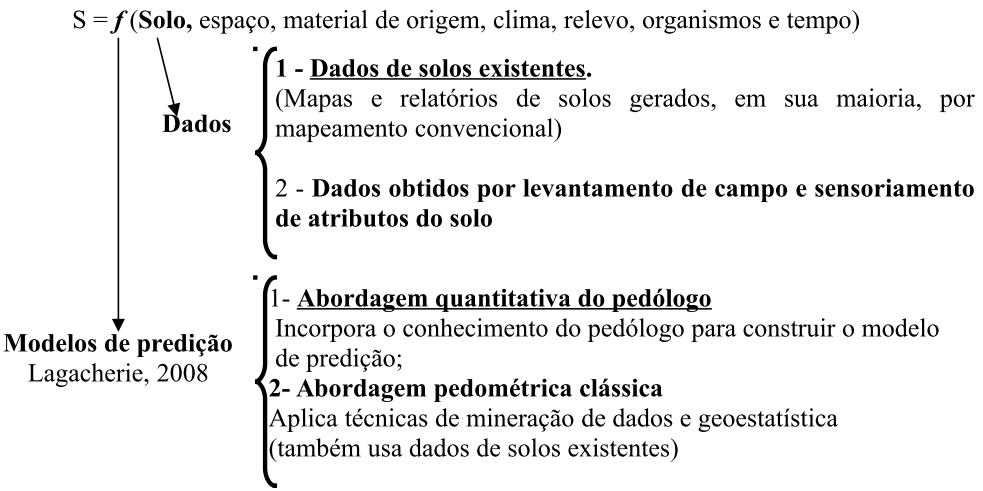
\includegraphics[width=\textwidth]{figuras/marcos-esquema}
   \caption{As possibilidades de interface entre o mapeamento convencional e o digital contextualizando no modelo SCORPAN}
   \label{fig:esquema}
 \end{center}
\end{minipage}
\end{figure*}
Quando o dado existente de solo é usado diretamente, esta interface se dá como sendo o fator solo. Nesse caso um exemplo seria a utilização de um mapa de
variabilidade espacial de um atributo do solo, considerado útil para discretização de classes ou mesmo a geração de mapa de outro atributo do solo. O mesmo dado de solo pode também gerar um modelo de predição ($f$), por exemplo, um modelo de regressão linear múltipla para predição espacial de um atributo (Água Disponível Total) a partir de outros atributos do solo (areia, argila, carbono) e de covariáveis (declividade, curvatura, índice topográfico de umidade). Nesse caso, a
mineração de dados é bastante útil para extrair ou ajudar a evidenciar padrões nestes dados e auxiliar na descoberta de conhecimento sobre solo e covariáveis. Esse conhecimento pode resultar em diversos produtos, tais como agrupamentos, hipóteses, regras, árvores de decisão, redes neurais e etc.\\
No segundo caso, o conhecimento do pedólogo é incorporado no modelo através de consulta direta, ou através da análise conjunta de mapas de solos e de covariáveis. Quando se consulta o pedólogo diretamente, o conhecimento pode ser incorporado através da construção de uma função de predição espacial ($f$), por exemplo, sistemas especialistas (implementação de regras de probabilidade condicional Bayesiana, lógica Fuzzy, e leis físicas simplificadas explicando a distribuição espacial de atributos do solo).\\
Outra forma de introdução do conhecimento de solos e covariáveis no MDS é a extração das relações solo/covariáveis diretamente no produto final de um levantamento de solos, no caso o próprio mapa. Nesse caso, por escolha ou indisponibilidade, não se consulta o pedólogo e sim o produto de seu modelo mental. O mapa, por refletir o modelo mental, é suficiente para extrair relações solo/covariáveis e construir um modelo de predição espacial. Um exemplo de extração desses padrões é a técnica da Área de Referência (AR).\\
De acordo com \cite{LagacherieEtAl:1995} muita pesquisa tem sido focada no uso inovativo de mapas de solos, tanto como uma fonte de dados para modelos de avaliação das terras ou como uma fonte adicional de informação para melhorar a eficiência de técnicas de interpolação, como a krigagem. Estes estudos tem demonstrado a
eficiência de mapas detalhados de solos (\textgreater{}1:25.000). No entanto, mapas detalhados não estão disponíveis em grande parte do território dos países, sobretudo no Brasil. Pensando em superar essa deficiência, \cite{Favrot:1981} propôs o método da Área de Referencia (AR). O objetivo desse método é caracterizar a cobertura de solos de regiões topograficamente e geologicamente identificáveis, denominadas ``pequenas regiões naturais''. O primeiro passo desse método consiste em efetuar o mapeamento detalhado de uma pequena, mas representativa área, de uma pequena região natural, a qual é denominada A.R.. Nesta A.R. caracterizam- se as principais classes de solos de toda a região e se estabelecem as regras de mapeamento. Esta primeira etapa facilita e acelera a etapa seguinte, a qual consiste na condução de novos trabalhos de mapeamento em áreas circunvizinhas. Na condução dos novos trabalhos de mapeamento, são levantados novos pontos de observação onde se esperam encontrar as mesmas classes de solos 
identificadas e mapeadas na A.R. Assim, também se espera poder fazer o delineamento dos limites de unidades de mapeamento a partir das regras de mapeamento preestabelecidas na A.R.\\
Quando se desenvolve mapeamento tendo como base o método da A.R., o que esta sendo testado é a hipótese de que é possível delimitar áreas (denominadas ``pequenas áreas naturais'') que englobem um número finito de classes de solos, as quais são recorrentes em associação umas com as outros na paisagem e formando um padrão repetitivo e identificável. Desta forma, uma A.R. propositalmente escolhida seria suficiente para identificar todas as classes de solos de uma área maior e também determinar suas relações espaciais. Segundo \cite{LagacherieEtAl:1995} a hipótese assumida no método da A.R. ainda precisa ser experimentalmente confirmado, embora já existam estudos, sobretudo na França, demonstrando que o método de A.R. é satisfatório. Ainda segundo \cite{LagacherieEtAl:1995}, os resultados obtidos na França
demonstram que os trabalhos efetuados utilizando A.R. tem reduzido a necessidade de trabalhos de campo, e que em geral menos de 10\% das unidades de solos encontradas nas novas áreas são diferentes daquelas estabelecidas nas A.R. Por outro lado, o mesmo autor observa que os ganhos de eficiência obtidos quando se aplicou a técnica de A.R. é obtida quando a equipe que faz os mapeamentos de outras áreas é a mesma que participou do trabalho da A.R. Assim, a desvantagem do método da A.R. é que a experiência obtida durante o mapeamento da área de referencia parece não ser ainda adequadamente explicitadas nos relatórios e mapas publicados, limitando sua transferência a outros pedólogos. Para contornar a limitação do método, \cite{LagacherieEtAl:1995} e outros pesquisadores, tem apresentado procedimentos computadorizados de levantamento de solos onde se procura reproduzir o raciocínio que um pedólogo experiente segue durante um levantamento realizado após uma pesquisa em uma área de referência.\\
De acordo com \cite{WalterEtAl:2007}, dois tipos de regras de conhecimentos de especialistas tem sido derivadas de mapas de solos, as quais são denominadas ``regras solo paisagem'' e `` regras de padrão de solos''. No primeiro caso (solo paisagem) utilizam-se como preditores os fatores do modelo SCORPAN, tais como derivadas do MDE e de sensores remotos para predizer classes de solos em lugares não visitados. Para a predição tem sido utilizados algorítimos como arvores de decisão \citep{Lagacherie:1992, LagacherieEtAl:1997, BuiEtAl:1999}, as quais fornecem um conjunto de regras de probabilidades de predição de unidades de mapeamento de solos.  No segundo caso (regras de padrões de solos), regras de padrões de distribuições de solos são capturadas nas áreas de referencia para inferência em uma área de interesse. Neste caso, utiliza-se como exemplo ilustrativo a ocorrência de três tipos de unidades de mapeamento, aqui denominadas A, B e C. Se o pedólogo observa
que na área de referencia, sistematicamente, a unidade de mapeamento C ocorre entra as unidades de mapeamento A e B, então cria-se uma regra de padrão de distribuição onde essa variação sistemática é transformada em regra de mapeamento. Assim, por exemplo, poder-se-ia determinar uma distância na qual, dado a presença da unidade C, encontrar-se-ia as probabilidades de ocorrência das unidades B e A. \cite{LagacherieEtAl:1995}, utilizou essa técnica no Valley of Herault no sul da França e considerou a técnica promissora para regiões onde padrões de distribuição de solos são identificáveis e recorrentes.\\
No Brasil a técnica de AR é ainda relativamente pouco aplicada. A técnica foi aplicada por \cite{TenCatenEtAl:2011} para mapear classes de solos no município de São Pedro do Sul-RS. Os autores concluíram que o MDS a partir de uma AR pode ser utilizado como alternativa ao mapeamento convencional para dimensões mais extensas da paisagem. A seleção de áreas de referência representativas da paisagem a ser mapeada é uma fase crucial para a adequada extrapolação das relações solo-paisagem, além da seleção de variáveis ambientais, as quais tenham forte relação com a pedogênese dos solos a serem mapeados.\\
Outro trabalho que utilizou a técnica de AR no Brasil foi o desenvolvido por \cite{Villela:2013}. O autor aplicou a técnica para mapear classes de solos sob floresta amazônica no município de Coari - AM. A partir de uma área de 7.900 hectares, a qual foi mapeada de forma convencional em escala detalhada (1:10.000), o autor desenvolveu funções discriminantes para mapear classes de solos de uma região no entorno com dimensões de 50.000 hectares, em escala 1:25.000, e de 116.000 hectares em escala 1:50.000. Os resultados de \cite{Villela:2013} e de \cite{TenCatenEtAl:2011} indicam que a técnica de AR é promissora. Os autores destacam a necessidade de desenvolver maiores estudos de validação e destacam a necessidade de avaliar a dimensão espacial da validade das extrapolações feitas a partir de uma área de referência.
\section{Demandas e desafios da interface}
Quando  avaliamos  as  possibilidades  de  interface,  dois  aspectos básicos se destacam, o primeiro refere-se à necessidade de um Sistemas de Gerenciamento de Banco de Dados de solos (SGBDsolos), e o segundo é a necessidade de aproximação entre diferentes gerações de pedólogos. A criação de um SGBDsolos é uma grande demanda, pois alem de permitir a organização e preservação do acervo de dados, permitirá o trabalho mais eficiente de mineração de dados por diversas instituições. No entanto, o assunto banco de dados é bastante complexo, pois envolve questões técnicas (modelagem do banco, software e hardware), jurídicas, disponibilidade e política de dados. No Brasil, apesar da lei de acesso a informação (Lei N° 12.527 de 18/11/2011), de modo geral, não existe a cultura de acesso à informação, inclusive para dados de solos. Na verdade, ate hoje não temos um SGBDsolos e são raros os arquivos de dados e mapas de solos que podem ser acessados. Os poucos exemplos de endereço na Internet onde é possível obter dados 
e mapas de solos, são:
\begin{enumerate}
\item \href{http://www.esalq.usp.br/gerd}{Esalq} - \underline{Fonte de dados}: RADAMBRASIL. 5.479 perfis de solo; 10.950 horizontes e 57 colunas com variáveis independentes. \underline{Formato}: .xls e .mdb;
\item \href{ftp://geoftp.ibge.gov.br/mapeamento_sistematico/banco_dados_georeferenciado_recursos_naturais/latlong/}{IBGE - latlong} ou \href{ftp://geoftp.ibge.gov.br/mapeamento_sistematico/banco_dados_georeferenciado_recursos_naturais/albers/}{IBGE - albers} - \underline{Fonte}: RADAMBRASIL (incorporado ao IBGE); \underline{Formato}: .pdf, shapefile; \underline{Tipo de dados}: mapas de solos, geomorfologia, geologia e vegetação.
\end{enumerate}
Os únicos dados e mapas parcialmente disponíveis são aqueles gerados pelo projeto RADAMBRASIL.\\
Com relação à aproximação entre diferentes gerações de pedólogos, é possível que exista em algumas instituições e em momentos específicos, no entanto, ainda é muito pouco expressiva diante da grande importância. O diálogo mais frequente e sistematizado permitirá a transmissão do conhecimento e definição de estratégias de mapeamento sistemático do Brasil.\\
Quanto mais nos aprofundamos na pesquisa em MDS notamos o quão vasto é a área, o que causa uma certa sensação de impotência diante de tantas áreas importantes para serem estudadas. Destaco aqui \underline{algumas} áreas que, além do ensino formal de solos, precisam ser utilizadas para aperfeiçoamento do MDS, são elas:
\begin{itemize}
\item Treinamento em modelagem matemática;
\item Desenvolvimento de software e bancos de dados;
\item Desenvolvimento e avaliação de sensores;
\end{itemize}
Cada uma dessas áreas possui várias subdivisões e por si demandam uma vida científica, logo dificilmente uma única pessoa domina eficientemente todas as áreas de conhecimento envolvidas no MDS. Assim, parece mais razoável investir no desenvolvimento de grupos interdisciplinares. ``\underline{Não é fácil achar um Michelangelo}''.
\section{Considerações finais}
O MDS é uma realidade no Brasil e representa a melhor alternativa para atender as demandas crescentes da sociedade por informações de solos. No entanto, ainda há um caminho longo a ser percorrido para que tenhamos um processo de mapeamento sistemático do território brasileiro através do MDS. Ainda precisamos criar protocolos mínimos para o MDS, formar mais profissionais na área, produzir materiais didáticos, fazer mais reuniões cientificas com diferentes gerações de pedólogos e, sobretudo, nos atirarmos na execução de mapas de solos no território Brasileiro. A prática constante nos permitira apresentar uma alternativa sólida de mapeamento para o Brasil.\\
O MDS é por natureza multidisciplinar, portanto, o seu desenvolvimento passa pela solidificação de trabalhos através de parcerias. Trabalhos em parcerias podem acelerar a geração de resultados práticos, no entanto, são mais complexos de serem gerenciados e exigem um grau de amadurecimento de pessoas e instituições bastante elevado. Um fato inquestionável, que denota o quanto ainda temos que avançar em termos de parceria nacional, é a não existência de um sistema de gerenciamento de banco de dados de solos do Brasil. Destaco aqui algumas características que considero essenciais para o sucesso das parcerias em MDS:
\begin{itemize}
\item Ter humildade para perceber a necessidade do trabalho em grupo;
\item Trocar o conhecimento para torná-lo disponível e aplicado;
\item Ter a visão de todo o processo de mapeamento digital de forma que não nos paralisemos nas inúmeras etapas entre o planejamento do mapeamento e a entrega do produto final;
\item Saber passar ao usuário como a informação de solo lhe pode ser útil.
\end{itemize}
Desde 2011 o Brasil possui uma Rede Brasileira de Mapeamento Digital em alta Resolução, congregando pesquisadores de vários estados e instituições. O fortalecimento dessa rede é o que temos de mais próximo de um trabalho em parceria em MDS.
\begin{footnotesize}
\begin{thebibliography}{99}
\bibitem[Bui et~al. (1999) Bui, Loughhead \& Corner]{BuiEtAl:1999}
E.N. Bui, A. Loughhead \& R. Corner (1999)
\newblock Extracting soil-landscape rules from previous soil surveys.
\newblock {\em Soil Research} 37: 495-508.
\bibitem[Burrough et~al. (1971) Burrough, Beckett, Jarvis]{BurroughEtAl:1971}
P.A. Burrough, P.H.T. Beckett \& M.G. Jarvis (1971)
\newblock The relation between cost and utility in soil survey (I--III).
\newblock {\em  Journal of Soil Science} 22: 359-394.
\bibitem[Favrot (1981) Favrot]{Favrot:1981}
J.C. Favrot (1981)
\newblock Pour une approche raisonnée du drainage agricole en France: La méthode des secteurs de référence.
\newblock {\em C.R. Académie d'Agriculture de France} 716-723.
\bibitem[Jenny (1941) Jenny]{Jenny:1941}
H. Jenny (1941)
\newblock Factors of soil formation - a system of quantitative pedology.
\newblock Dover Publications, New York. 281p.
\bibitem[Lagacherie (1992) Lagacherie]{Lagacherie:1992}
P. Lagacherie (1992)
\newblock Formalisation des lois de distribution des sols pour automatiser la cartographie pédologique à partir d'un secteur pris comme référence.
\newblock {\em Thesis (PhD in Soil Science)} 175p.
\bibitem[Lagacherie et~al. (1995) Lagacherie, Legros \& Burfough]{LagacherieEtAl:1995}
P. Lagacherie, J. P. Legros \& P. Burfough (1995)
\newblock A soil survey procedure using the knowledge of soil pattern established on a previously mapped reference area.
\newblock {\em Geoderma} 65: 283-301.
\bibitem[Lagacherie \& Holmes (1997) Lagacherie \& Holmes]{LagacherieEtAl:1997}
P. Lagacherie \& S. Holmes (1997)
\newblock Addressing geographical data errors in a classification tree for soil unit prediction.
\newblock {\em International Journal of Geographical Information Science} 11: 183-198.
\bibitem[Lagacherie \& McBratney (2007) Lagacherie \& McBratney]{LagacherieEtal:2007}
P. Lagacherie, A.B. McBratney (2007)
\newblock Spatial soil information systems and spatial soil inference systems: perspectives for Digital Soil Mapping.
\newblock {\em Digital Soil Mapping, an introductory perspective. Developments in soil science} 31:3-24.
\bibitem[Lagacherie (2008) Lagacherie]{Lagacherie:2008}
P. Lagacherie (2008)
\newblock Digital Soil Mapping: State of the Art.
\newblock {\em Digital Soil Mapping with Limited Data}, pp.3-14.
\bibitem[McBratney et~al. (2003) McBratney, Mendonça-Santos, Minansny]{McBratneyEtAl:2003}
A.B. McBratney, M.L. Mendonça-Santos, B. Minansny (2003)
\newblock On Digital Soil Mapping.
\newblock {\em Geoderma} 117:3-52.
\bibitem[Mendonça-Santos \& Santos (2007) Mendonça-Santos \& Santos]{Mendonca-SantosEtAl:2007}
M.L. Mendonça-Santos, H.G. Santos (2007)
\newblock The state of the art of Brazilian soil mapping and prospects for digital soil mapping.
\newblock {\em Developments in Soil Science} 31:39-55.
\bibitem[Scull et~al. (2003) Scull, Franklin, Chadwick, Mcarthur]{ScullEtAl:2003}
P. Scull, J. Franklin, O.A. Chadwick, D. Mcarthur (2003)
\newblock Predictive soil mapping: a review.
\newblock {\em Progress in physical geography} 27:171-197.
\bibitem[Ten Caten et~al. (2011) Ten Caten, Dalmolin, Pedron, Mendonça-Santos]{TenCatenEtAl:2011}
A. Ten Caten, R.S.D. Dalmolin, F.A. Pedron, M.L. Mendonça-Santos (2011)
\newblock Extrapolação das relações solo-paisagem a partir de uma área de referência.
\newblock {\em Ciência Rural} 41: 812-816.
\bibitem[Villela (2013) Villela]{Villela:2013}
A.L.O. Villela (2013)
\newblock Mapeamento Digital de Solos da Formação Solimões - Urucu, AM.
\newblock {\em Thesis (PhD in Agronomy-Soil Science)} 110p.
\bibitem[Walter et~al. (2007) Walter, Lagacherie, Follain]{WalterEtAl:2007}
C. Walter, P. Lagacherie, S. Follain (2007).
\newblock Integrating pedological knowledge into Digital Soil Mapping
\newblock {\em Digital Soil Mapping, an introductory perspective. Developments in soil science} 31:281-300.
\end{thebibliography}
\end{footnotesize}
\address{Marcos Bacis Ceddia\\
  Universidade Federal Rural do Rio de Janeiro\\
  \url{www.aguaesolos.net}\\
  \email{marcosceddia@gmail.com}}
\end{article}

\begin{article}
   \title{Entrevista}
\subtitle{com Michele Duarte de Menezes}
\maketitle
\begin{wrapfigure}{l}{0.15\textwidth}
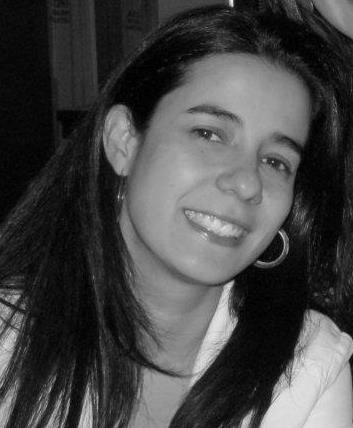
\includegraphics[width=0.15\textwidth]{figuras/foto-michele.png}
\end{wrapfigure}
Nesta edição da \textit{Newsletter} da Comissão de Pedometria da Sociedade Brasileira de Ciência do Solo, entrevistamos a Professora Doutora Michele Duarte de Menezes para falar um pouco sobre a Pedometria, suas potencialidades, dificuldades e perspectivas futuras no Brasil. A Dra. Michele atualmente é professora da disciplina de  Mapeamento Digital de Solos e Pedologia Aplicada na Universidade Federal Rural do Rio de Janeiro (UFRRJ). Sua formação pós ensino médio foi realizada na Universidade Federal de Lavras (UFLA), contemplando graduação em Agronomia, mestrado e doutorado em Ciência do Solo na área de Gênese, Morfologia e Classificação dos Solos. Realizou parte do seu doutorado na Purdue University (Estados Unidos). Publicou recentemente um artigo discorrendo sobre a importância da integração entre o conhecimento de campo do pedólogo e uso de ferramentas  estatísticas na predição de classes e propriedades de solos para a produção mais rápida de mapas de solos com acurácia das informações \citep{MenezesEtAl:2013}.\\
\\
\textbf{Pedometria} - O que levou você a se interessar e estudar sobre o Mapeamento Digital de Solos (MDS) e em especial temas relacionados a pedometria?\\
\\
\textbf{Michele} - Tanto no mestrado (início em 2005) quanto no doutorado, minhas atividades envolveram levantamento de solos e suas interpretações. Já no início do mestrado, os sistemas de informação geográficas e os modelos digitais de elevação começaram a se tornar mais acessível. Aliado a isso, e com o intuito de tentar melhorar os mapas de solos, comecei a ler inicialmente sobre mapeamento digital. Lembro-me que o primeiro material que li em português, foi um documento da EMBRAPA intitulado Mapeamento Digital de Classes e Atributos de Solos - métodos, paradigmas e novas técnicas \citep{MendoncaSantosEtAl:2003}. Esse documento traz um resumo sobre diversas técnicas pedométricas. Comecei então a cursar disciplinas e testar tais técnicas durante o meu período de treinamento.\\
\\
\textbf{Pedometria} - Quais são os projetos de pesquisa que você está desenvolvendo na área de MDS?\\
\\
\textbf{Michele} - Os projetos que tenho participado envolvem mapeamento de solos e seus atributos. Sob o ponto de vista de técnicas, temos empregado principalmente técnicas geoestatísticas (krigagem ordinária e krigagem combinada com regressão) e lógica \emph{fuzzy} (Figura \ref{fig:tecnicas}) aliada ao conhecimento \emph{expert}. Além disso, as pesquisas envolvem também o desenvolvimento de funções de pedotransferência, o uso sistemas de informação geográfica e geomorfometria.\\
\\
\begin{figure}[htbp]
\centering
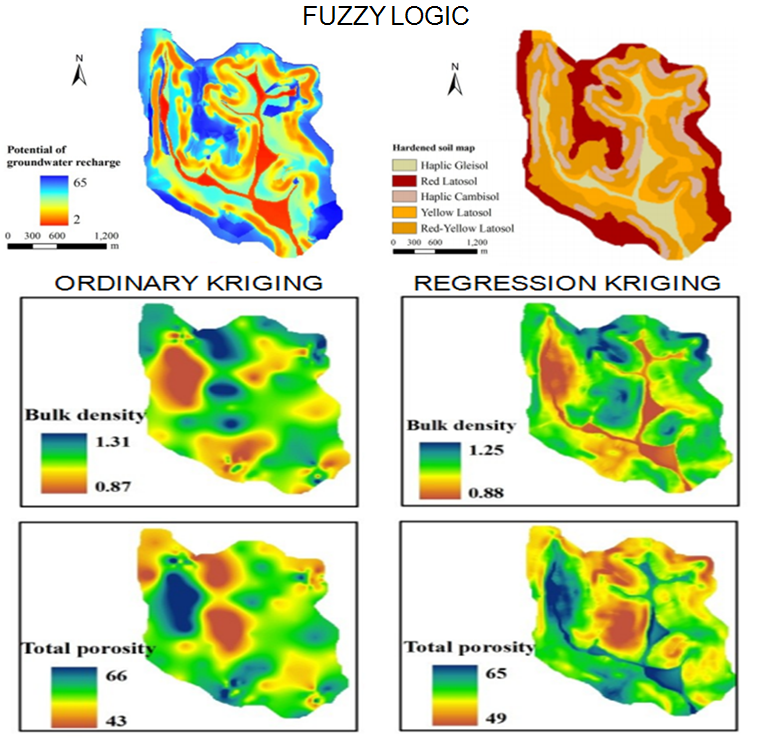
\includegraphics[scale=0.8]{figuras/tecnicas-predicao}
\caption{Técnicas de predição de atributos e classes de solos. Fonte: \cite{Menezes:2011}.}
\label{fig:tecnicas}
\end{figure}
\noindent \textbf{Pedometria} - O que você acha do cenário atual da pedometria no Brasil e qual o cenário que você vivenciou no seu doutorado sandwich em Purdue University nos EUA?\\
\\
\textbf{Michele} - Atualmente, tenho percebido um crescente interesse sobre a pedometria, por pessoas de diversas áreas do conhecimento da Ciência do Solo e outras áreas afins. No caso da UFRRJ, por exemplo, todas as disciplinas que envolvem técnicas pedométricas ou geotecnologias são muito procuradas na pós-graduação. Já nos Estados Unidos, o cenário foi um pouco diferente, pois eles já possuíam levantamento de solos em escalas mais detalhadas para grande parte do país, além de diversas interpretações a partir deles. A aquisição covariáveis ambientais para a predição é muito mais facilitada, como por exemplo, MDEs em elavada resolução gratuitamente disponíveis. Mais especificamente para o cenário de Purdue, as pesquisas estavam focadas principalmente na atualização dos mapas de solos já existentes, ou mesmo buscando gerar informações numéricas e continuamente distribuídas a partir do legado de solos (conhecimento tácito ou técnicas de mineração de dados).\\
\\
\textbf{Pedometria} - Qual a sua opinião a respeito da pedometria como uma disciplina nos cursos de Graduação e em especial nos Programas de Pós-Graduação na área de solos no Brasil?\\
\\
\textbf{Michele} - A pedometria tem um caráter multidisciplinar: eis um grande desafio para os cursos. A interação entre professores de diversas áreas do conhecimento é necessária. Além disso, vejo que existem muitos pré-requisitos acerca das técnicas de predição. Recentemente, foi ofertada aqui na UFRRJ uma disciplina chamada Métodos e Técnicas de Mapeamento Digital de Solos, ministrada pelos pesquisadores da EMBRAPA Solos Waldir de Carvalho Júnior, César da Silva Chagas, com minha colaboração. Diversas técnicas estatísticas e geostatísticas foram abordadas em aula, e um trabalho final usando uma base de dados real foi um dos requisitos. Percebi que os alunos tiveram dificuldade desde a formatação da base de dados, pois requeria um conjunto de operações em sistemas de informação geográfica, o que consiste em uma disciplina a parte. Outra dificuldade está relacionada à compreensão das técnicas em si (matemática, estatística e geostatística), o que exige muita leitura e compreensão mínima da linguagem 
matemática, onde teríamos talvez outra disciplina. Se formos pensar nas covariáveis ambientais, o uso do sensoriamento remoto é amplamente necessário, temos então mais uma nova disciplina complementar. Esses são apenas alguns exemplos que mostram que o desafio está em lidar efetivamente com esta multidisciplinaridade. Infelizmente, o processo de seleção dos programas de Pós-Graduação em Ciência do Solo estão cada vez mais específicos, dificultando o ingresso de alunos graduados em Matemática, Sistemas de Informação, Ciência da Computação, entre outros, o que seria salutar para o ensino e desenvolvimento da pedometria.\\
\\
\textbf{Pedometria} - Pela sua experiência na área de MDS, quais as principais dificuldades e desafios encontrados para os pesquisadores brasileiros desenvolverem seus trabalhos?\\
\\
\textbf{Michele} - Tanto para o pesquisador em MDS, quanto para outras áreas, as dificuldades são muito semelhantes, e geralmente de ordem burocrática. No entanto, de modo geral, os recursos disponíveis são crescentes para pesquisa. Pensando nas dificuldades do pesquisador em MDS, o foco no estabelecimento de infraestrutura é necessário, para um futuro impacto na qualidade dos produtos gerados. Nesse sentido, o desenvolvimento de um banco de dados de solos bem como a obtenção e livre disponibilização de informações ou mapas que representem covariáveis ambientais \ref{figure:covar}, em escalas mais detalhadas ou elevada resolução (exemplo: modelos digitais de elevação, mapas geológicos, uso e cobertura do solo, entre outros) são mais urgentes. Um dos desafios consiste na geração de novos dados de solos, como novas campanhas de campo, acompanhadas de técnicas de otimização amostral e o avanço do uso do sensoriamento remoto.\\
\\
\begin{figure}[htbp]
\centering
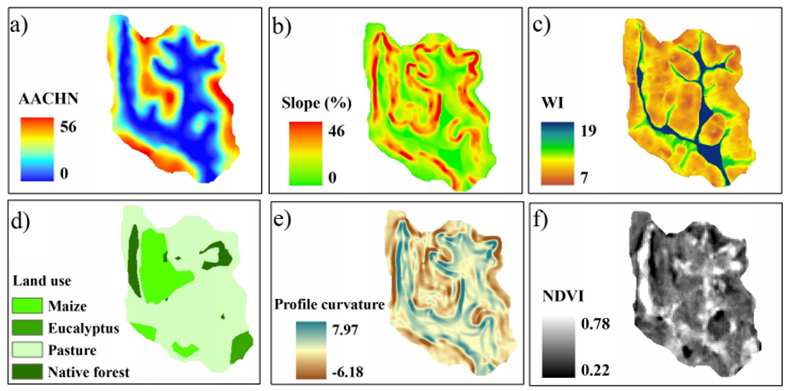
\includegraphics[scale=0.8]{figuras/covariaveis-ambientais}
\caption{Exemplos de covariávies ambientais utilizadas na predição de atributos do solo. Fonte: \cite{Menezes:2011}.}
\label{figure:covar}
\end{figure}
\noindent \textbf{Pedometria} - Você vê a pedometria como uma ferramenta promissora para ser utilizada na obtenção de informações de qualidade sobre solos e assim abastecer banco de dados de solos brasileiros?\\
\\
\textbf{Michele} - Sem dúvida a pedometria tem elevado potencial para geração de dados para um banco de dados. Acredito também no potencial dos pesquisadores brasileiros para implementar tais técnicas e gerenciar os dados. No entanto, o principal entrave não está no uso de técnicas, mas sim na burocracia acerca da política de dados no Brasil. Talvez por isso não tenhamos um banco de dados para todo território brasileiro até então.\\
\\
\textbf{Pedometria} - Qual a sua opinião a respeito da interdisciplinaridade nos grupos de pesquisa em MDS para desenvolver trabalhos de qualidade e que contribuam para meio científico? Na sua opinião, existe interdisciplinaridade nos grupos de pesquisa do Brasil? Sim ou Não? Por quê?\\
\\
\textbf{Michele} - A interdisciplinaridade atualmente é um desafio para várias áreas do conhecimento, e para o MDS não é diferente. Contudo, a interdisciplinaridade ou mesmo a integração entre diferentes órgãos, e não apenas de pesquisa, ainda é pouco efetiva no Brasil. Dentre vários motivos, a falta de efetividade é herdada da estrutura organizacional das universidades, além do fato de que professores não recebem treinamento para desenvolvimento de trabalhos interdisciplinares. Conheço alguns poucos projetos de pesquisa que buscam integração com diferentes áreas. Esta parceria deveria envolver as Universidades, IBGE, INPE, CPRM, EMBRAPA entre outros órgãos.\\
\\
\textbf{Pedometria} - Qual a sua opinião a respeito da abordagem e discussão da pedometria e do MDS no último Congresso Brasileiro de Ciência do Solo? Esses temas estão ganhando mais espaço nos eventos científicos de solos? Qual a situação do interesse do público leitor por temas relacionados a pedometria?\\
\\
\begin{figure}[htbp]
\centering
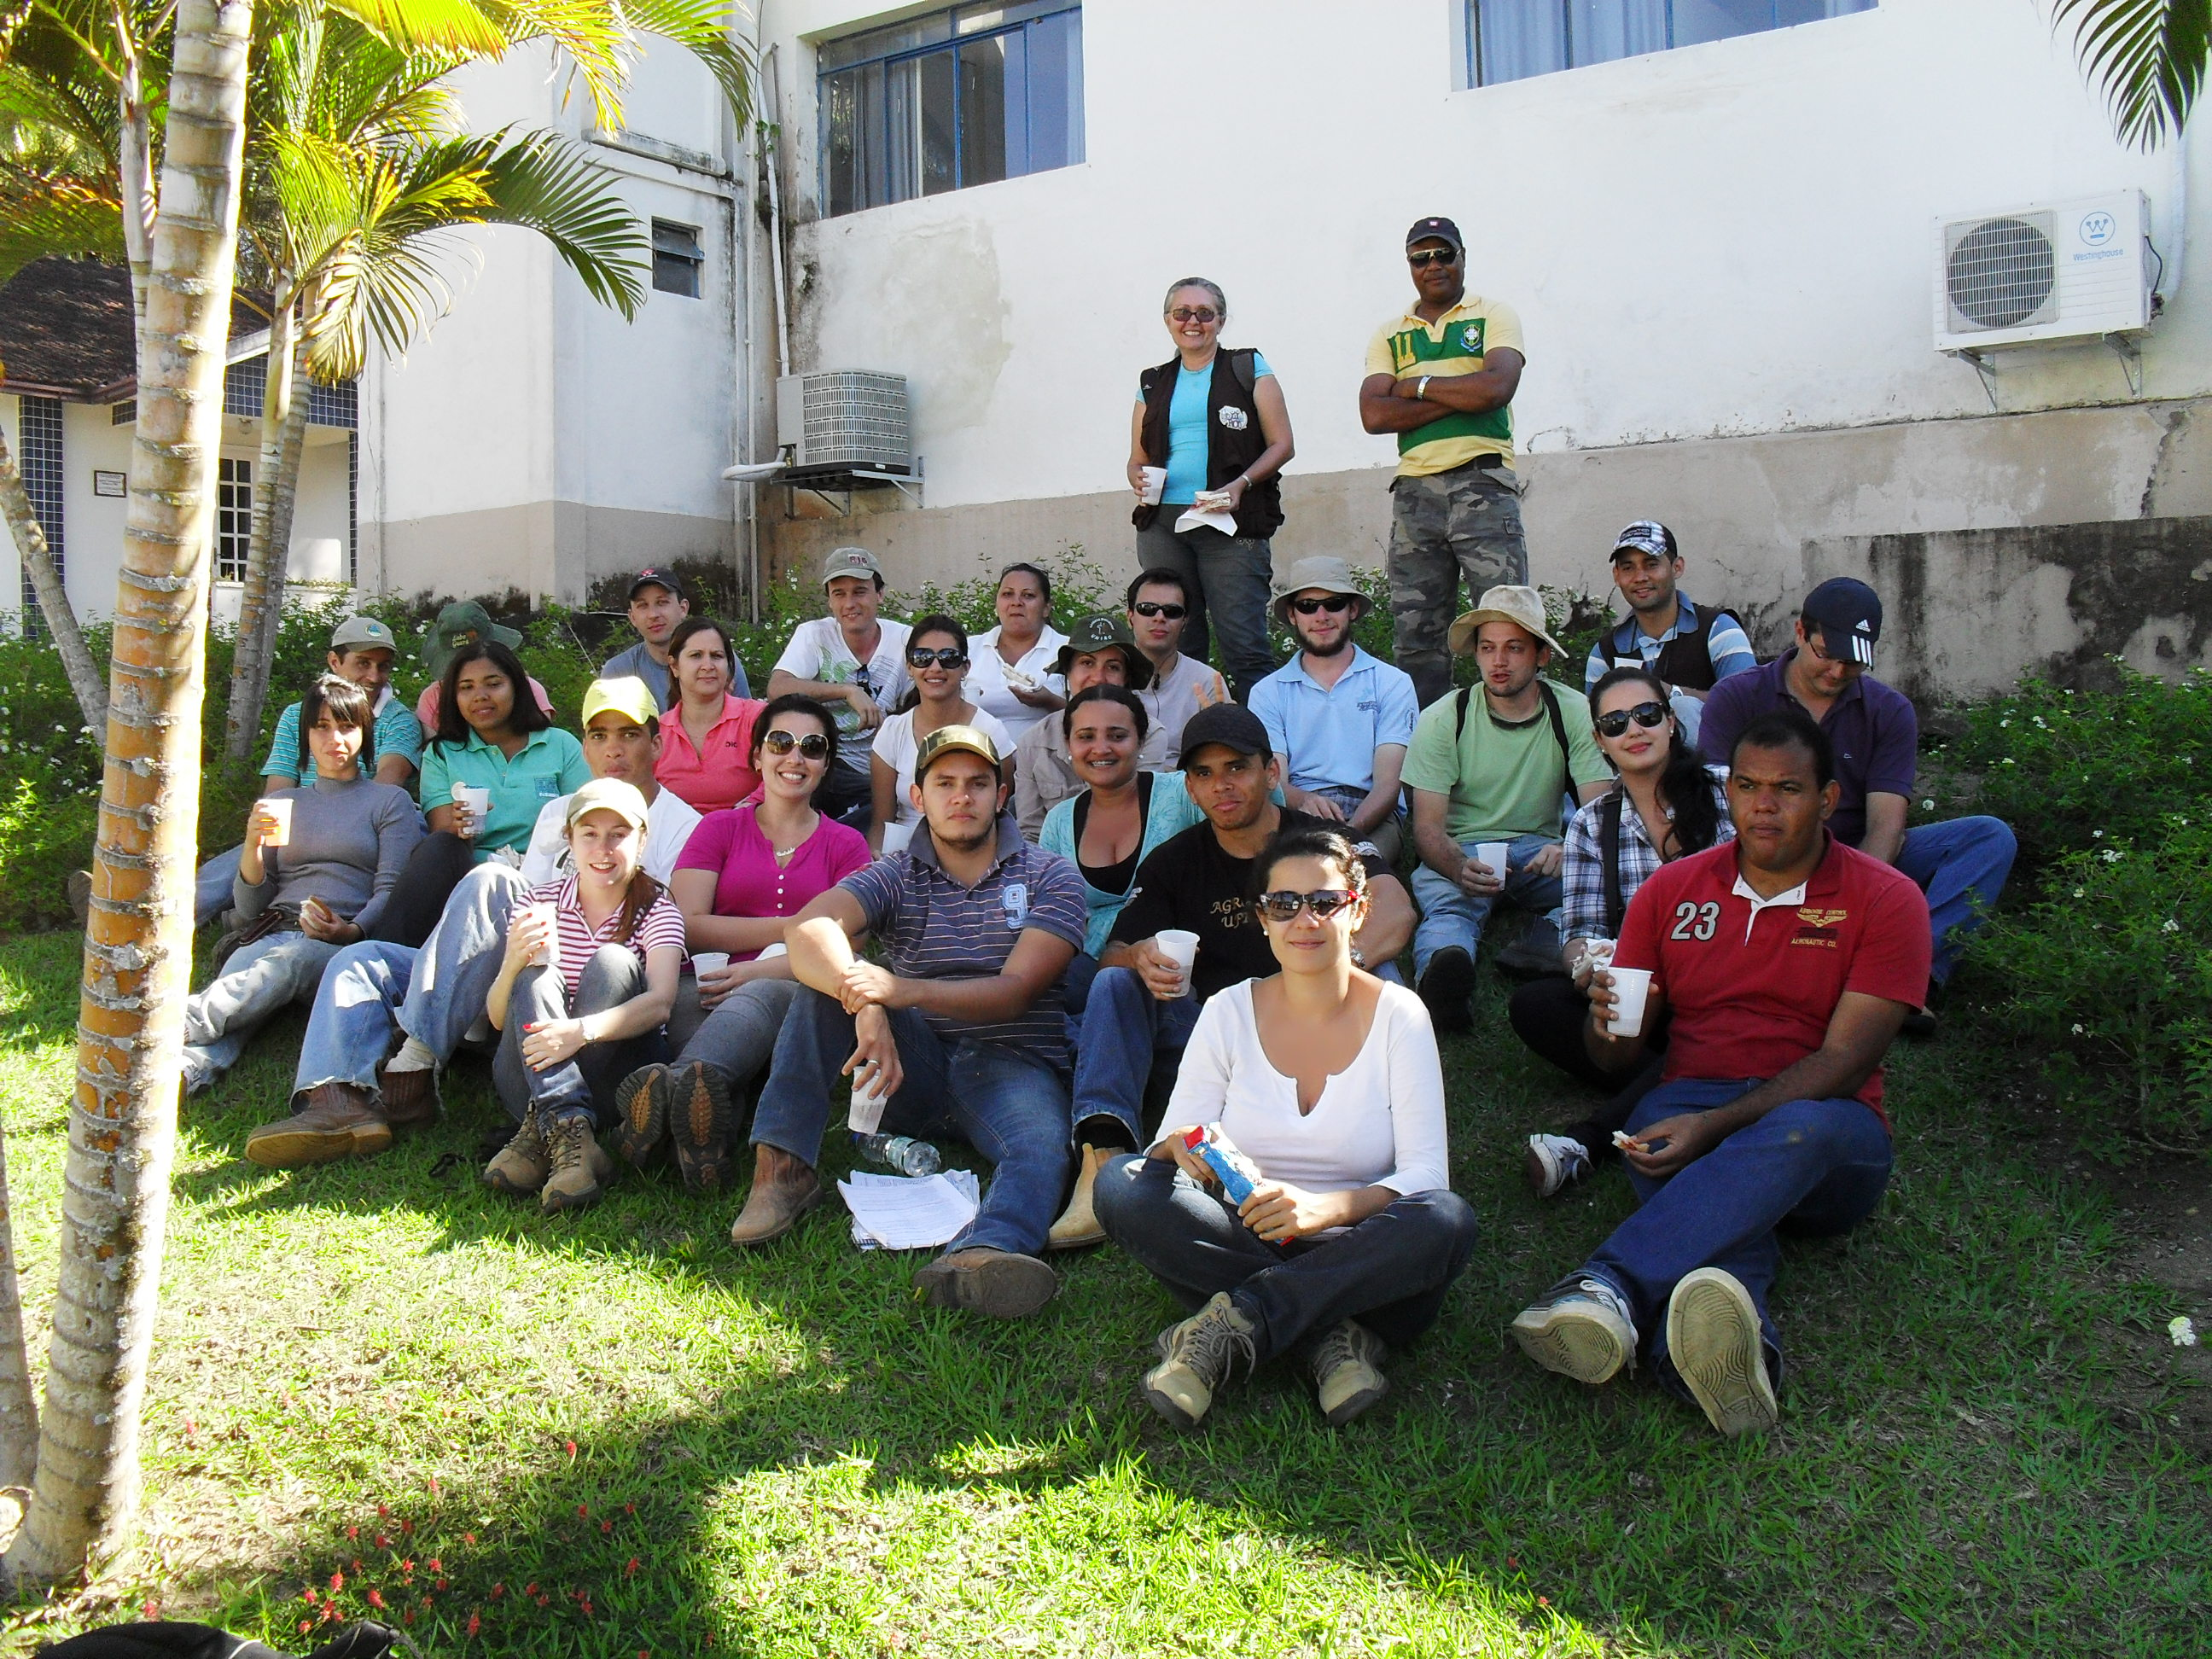
\includegraphics[scale=0.8]{figuras/michele-viagem}
\caption{A Dra. Michele (primeiro plano) acompanhando a prova de campo da disciplina de Formação e Caracterização do Solo da UFRRJ.}
\label{figure:covar}
\end{figure}
\noindent \textbf{Michele} - Creio que um dos assuntos mais comentados durante o Congresso desde ano foi a respeito da pedometria e o MDS, o que mostra um ganho de espaço nos eventos científicos ou mesmo enquanto linhas de pesquisa. Algumas palestras foram muito elucidativas, e espero que tenham acabado com alguns mitos ainda recorrentes acerca do MDS. Sim, os trabalhos de campo são de extrema importância ao mapeamento digital de solos. Não há dúvidas de que o conhecimento da Pedologia, Geomorfologia, Geologia, entre outras áreas, são fundamentais para o MDS e pedometria. Não, a pedometria não tem intuito de substituir a Pedologia, são áreas complementares ou afins. O próprio termo pedometria está relacionado à Pedologia (pedo), e metria está relacionada à parte da mensuração, a partir de métodos mais quantitativos (matemáticos e estatísticos).\\
A respeito do público leitor, creio que o interesse a respeito da pedometria tem crescido, principalmente entre pesquisadores e alunos de pós-graduação. Ao público em geral de outras áreas, acredito que soluções ambientais ou aplicações mais técnicas são mais interessantes.
\begin{footnotesize}
\begin{thebibliography}{99}
\bibitem[Mendonça-Santos \& Santos (2003) Mendonça-Santos \& Santos]{MendoncaSantosEtAl:2003}
M.L. Mendonça-Santos, H.G. Santos (2003)
\newblock Mapeamento digital de classes e atributos de solos: métodos, paradigmas e novas técnicas.
\newblock {\em Documentos} 55, 19p.
\bibitem[Menezes et~al. (2013) Menezes, Silva, Owens, Curi]{MenezesEtAl:2013}
M. D. Menezes, S. H. G. Silva, P. R. Owens, N. Curi (2013)
\newblock Digital soil mapping approach based on fuzzy logic and field expert knowledge.
\newblock {\em Ciência e Agrotecnologia} 37: 287-298. [\url{http://dx.doi.org/10.1590/S1413-70542013000400001}]
\bibitem[Menezes (2011) Menezes]{Menezes:2011}
M. D. Menezes (2011)
\newblock Levantamento pedológico de hortos florestais e mapeamento digital de atributos físicos do solo para estudos hidrológicos.
\newblock {\em Tese de doutorado, Universidade Federal da Lavras}, 225p.
\end{thebibliography} 
\end{footnotesize}
\address{Jean Michel Moura-Bueno\\
  Universidade Federal de Santa Maria\\
  \email{bueno.jean1@gmail.com}}

\end{article}

\begin{article}
   \title{Disciplina ``Métodos e Técnicas de Mapeamento Digital de Solos''}
\author{por Waldir de Carvalho Junior, Cesar da Silva Chagas e Michele Duarte de Menezes}
\maketitle
Em função da demanda de uma disciplina sobre o tema junto ao programa de pós-graduação do Departamento de Solos da UFRRJ, fomos solicitados a organizar uma  disciplina abordando o tema de mapeamento digital de solos (MDS) como Tópicos Especiais em Ciência do Solo. Inicialmente, foram realizadas duas reuniões com as Profas. Michele Duarte e Lucia Anjos para definição de uma estratégia para a disciplina e a estrutura para os alunos.\\
Ao todo 15 alunos de pós-graduação se inscreveram, sendo 10 do Departamento de Ciência do Solo e cinco de outros departamentos. Do total de matriculados apenas três alunos não concluíram a disciplina.\\
A disciplina, que na UFRRJ é trimestral (junho a agosto de 2013), teve ao todo 14 aulas com mais duas aulas extras no mês de setembro, perfazendo um total de 56 horas/aula, tempo considerado suficiente para apresentar aos alunos aspectos teóricos e práticos dos principais métodos de predição utilizados no MDS.\\
Inicialmente,  a disciplina apresentou uma breve teoria introdutória sobre mapeamento de solos, tipos e utilizações. Para nivelar os conhecimentos, foram apresentados alguns conceitos básicos de geoprocessamento, úteis para aplicação em mapeamento digital.\\
Uma das premissas do curso foi a utilização de softwares livres e quanto aos equipamentos de hardware, foi solicitado aos alunos que utilizassem seus próprios laptops/ notebooks.\\
A estratégia funcionou a contento já que os alunos puderam acompanhar satisfatoriamente todas as aulas práticas do curso. No entanto, vale ressaltar que  é necessária uma configuração mínima de hardware, de modo que todos os processamentos sejam realizados em tempo hábil durante as aulas.\\
\\
\begin{figure}[htbp]
   \centering
   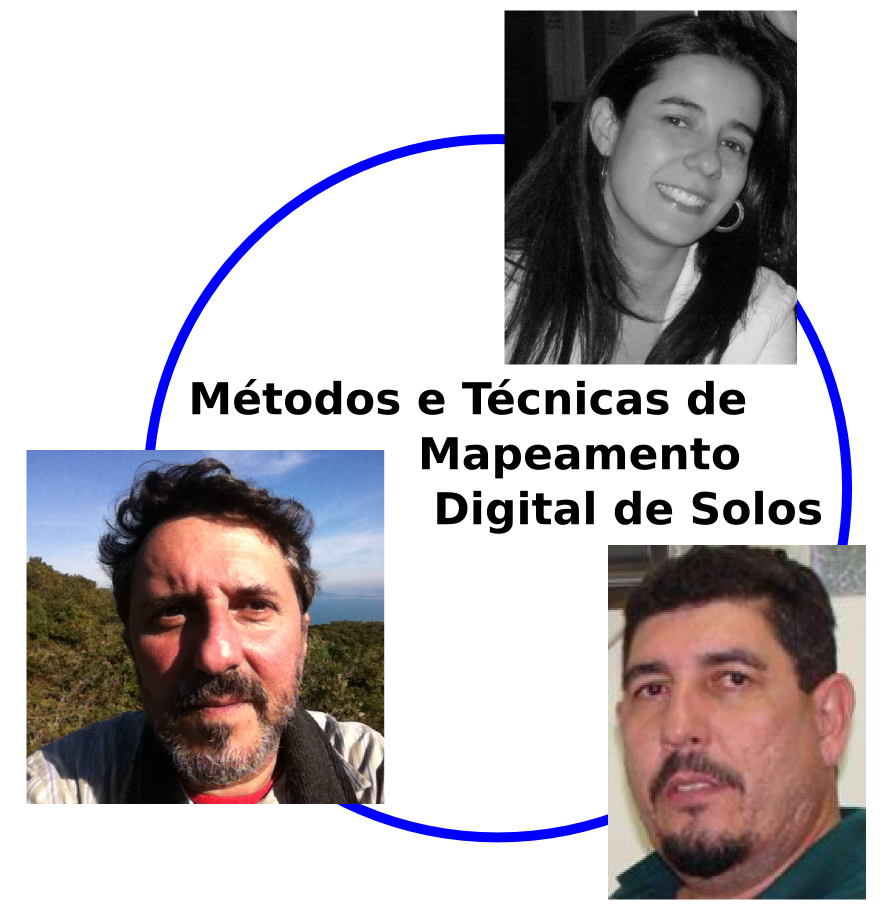
\includegraphics[width=0.95\linewidth]{figuras/trio}
   \caption{O trio de professores.}
   \label{fig:foto-trio}
\end{figure}
\noindent Os seguintes softwares livres foram utilizados: SAGA GIS, R e SoLim. Inicialmente, foram dados aos alunos noções básicas destes softwares, para que eles se habituassem com os mesmos.\\
Nos procedimentos das aulas práticas foi utilizado um conjunto de dados com 101 perfis de solos analisados com resultados de argila e carbono do horizonte A, pertencentes ao projeto Corredor Ecológico do COMPERJ na Bacia do Rio Guapi-Macacu no Estado do Rio de Janeiro.\\
\\
\begin{figure}[htbp]
   \centering
   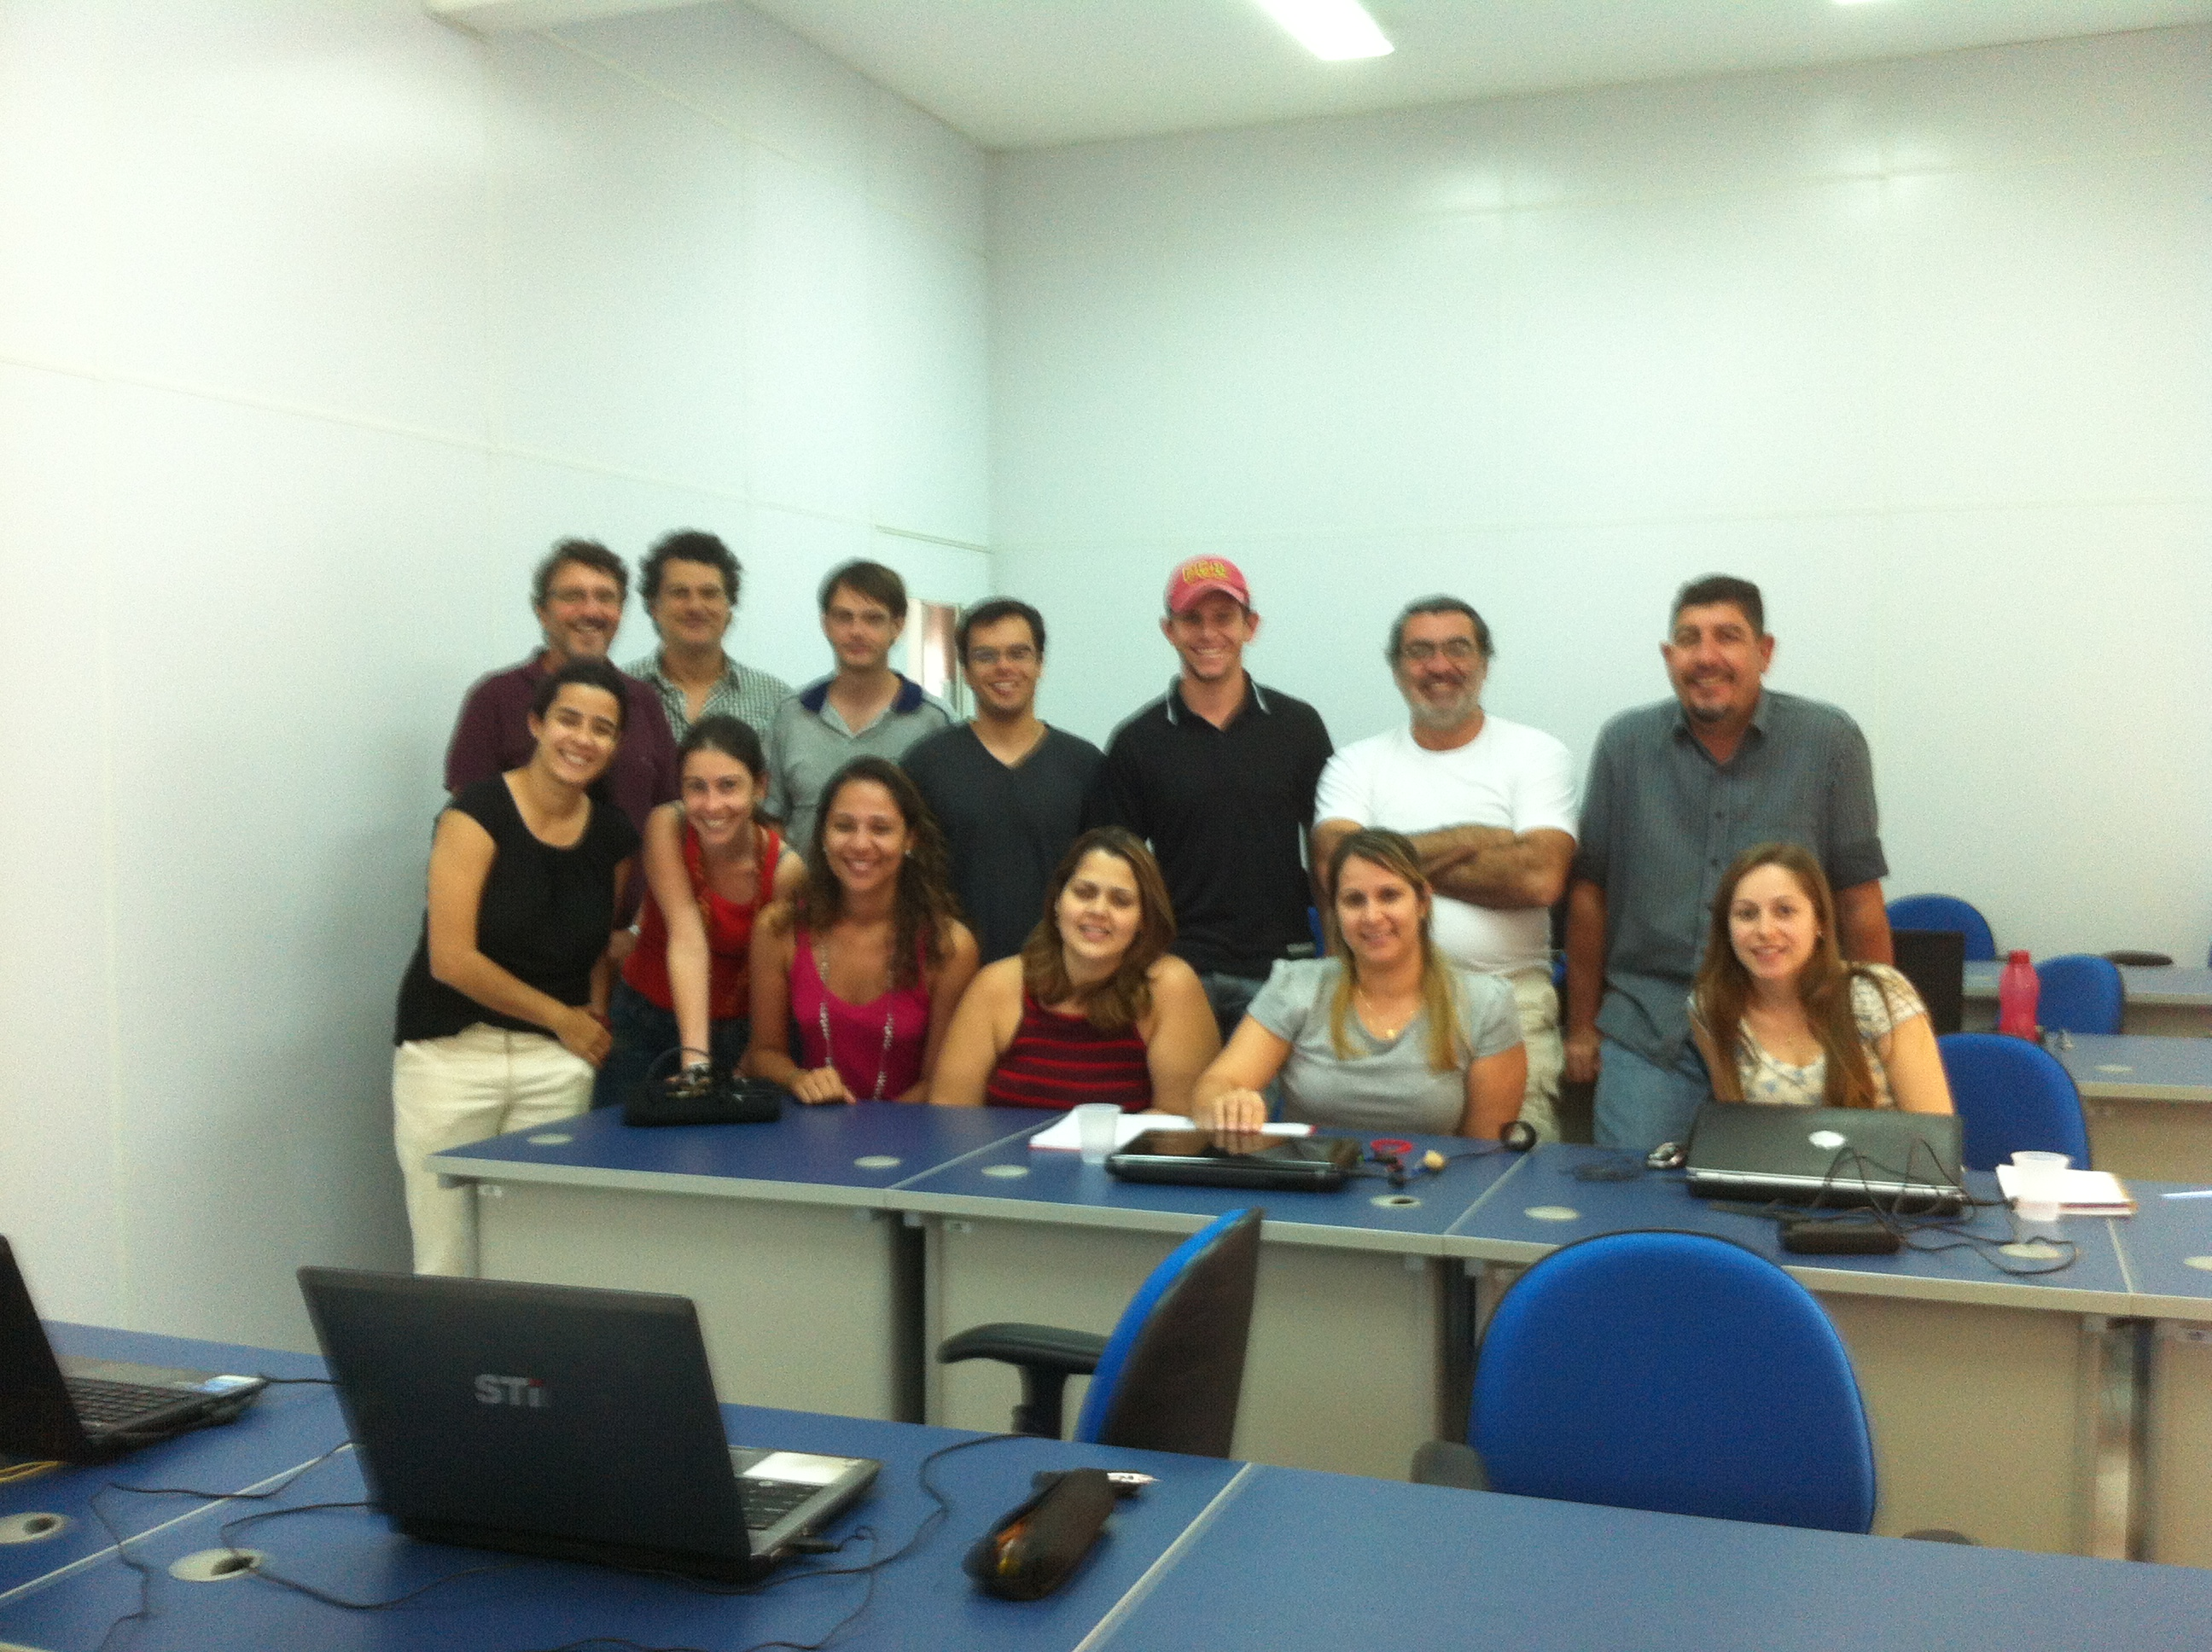
\includegraphics[width=0.95\linewidth]{figuras/foto-waldir.jpg}
   \caption{Foto do grupo.}
   \label{fig:foto}
\end{figure}
\noindent As aulas contemplaram os seguintes temas: Introdução ao Mapeamento Digital de Solos (MDS), Introdução ao uso de ferramentas computacionais livres e abertas para MDS, Variáveis e Covariáveis usadas Mapeamento Digital de Solos, Cálculo de Covariáveis Ambientais usadas em MDS usando ferramentas de SIG, Introdução a Modelagem para MDS, Utilização do SAGA GIS e R na modelagem para MDS, Modelos Lineares Simples e Múltiplos eaplicações do R, Modelos de Árvores de Decisão e Regressão e aplicação no R, Modelos do tipo Random Forest logísticos e de regressão, Random Forest e aplicações no R, Conceitos e Estruturas de Redes Neurais Artificiais, Construção e Aplicação de Redes Neurais Artificiais no pacote RSNNS no R, Introdução aos sistemas SoLIM e Knowledge, Experiências com softwares SoLIM e Knowledge, Mapeamento digital de classes de solos com Redes Neurais, Teoria de Geoestatística e sua interação com mapeamento digital de solos, Aplicação de Geoestatística para mapeamento de atributos do solo, Teoria de cokrigagem 
e regressão-krigagem sua interação com mapeamento digital de solos, Aplicação de de cokrigagem e regressão-krigagem para mapeamento de atributos do solo no R.\\
A disciplina contou também com a participação especial do Dr. Prof. Phillip Owens da Purdue University  que falou sobre sua experiência com mapeamento digital de solos.\\
Como avaliação final da disciplina foi proposto um trabalho prático com dados oferecidos ou próprios dos alunos, em formato de artigo, seguindo as normas da RBCS, a ser entregue até o final de setembro.\\
No final do curso, foi solicitado aos alunos que avaliassem o mesmo, através de um questionário. O resultado da avaliação do curso pelos alunos  mostrou pontos positivos e negativos, detalhados a seguir. A primeira pergunta era: ``Quanto à carga horária, foi satisfatória ou não? A distribuição (04 horas/semana) foi conveniente?''. As respostas em sua maioria (11) foi positiva às duas questões (carga horária e distribuição), entretanto  três alunos sugeriram uma carga horária maior. Apenas um aluno sugeriu que houvesse duas aulas por semana com duas horas cada.\\
A segunda questão foi: ``Em sua avaliação, quais foram as principais dificuldades para acompanhar o curso?'', com as opções de didática, material didático (dados e softwares apresentados durante o curso), carga horária e distribuição, hardware, software, instalações (estrutura), outras (especificar).  A principal dificuldade apontada pelos alunos foi ``software'', seguido por ``hardware'' e ``conhecimentos em mapeamento de solos'' (contida na opção outras). As opções de ``material didático (dados e softwares apresentados durante o curso)'' e ``carga horária e distribuição'' aparecem a seguir. Não foram mencionados a ``didática'' , nem ``instalações (estrutura)''.\\
A terceira questão foi: ``Você acredita que alguma das disciplinas da pós-graduação ou algum conhecimento específico deveriam ser pré-requisitos para o curso? Quais?'' A maioria disse que sim, mas sem que o termo ``pré-requisito'' seja empregado, ficando apenas como sugestão para futuros alunos. Os alunos apontaram as seguintes disciplinas em ordem decrescente de importância: Estatística e Geoestatística Geoprocessamento/SIG, Pedologia, classificação e levantamento de solos, básico de R.\\
A última questão diz: ``A forma de avaliação (trabalho prático apresentado em formato de artigo) está coerente com o curso? Uma apresentação do trabalho para os colegas é interessante?'' A maioria respondeu ``sim'' às duas indagações.\\
A experiência desta primeira disciplina foi  positiva e nos permitiu montar uma estrutura que pode ser aperfeiçoada para uma possível reapresentação da disciplina no próximo ano ou até mesmo em outra instituição que esteja interessada no curso. O esforço de preparação das aulas foi compensado também com nosso aprendizado.\\
A oferta da disciplina de MÉTODOS E TÉCNICAS DE MAPEAMENTO DIGITAL DE SOLOS supriu uma demanda na pós-graduação do Departamento de Ciência do Solo da UFRRJ. Por não se tratar de uma disciplina regular, a procura pode ser considerada satisfatória, com 15 alunos inicialmente matriculados e 12 concluindo o curso.\\
Temos agora um conjunto de dados estruturados, que pode servir de ponto de partida para uma nova oferta desta disciplina.\\

\address{Waldir de Carvalho Junior\\
Embrapa Solos\\
\url{www.cnps.embrapa.br}\\
\email{Waldir.Carvalho@embrapa.br}}\\
\address{Cesar da Silva Chagas\\
Embrapa Solos\\
\email{Cesar.Chagas@embrapa.br}}\\
\address{Michele Duarte de Menezes\\
Universidade Federal Rural do Rio de Janeiro\\
\email{michele\_duarte@ig.com.br}}
%%% Local Variables: 
%%% mode: latex
%%% TeX-master: documento-principal.tex
%%% End:
\end{article}

\begin{article}
   \title{Mapeamento Digital no Ensino de Ciência do Solo}
\subtitle{Capacitação e Perspectivas para o Futuro do Levantamento de Solos no País}
\author{por Helena Saraiva Koenow Pinheiro}
\maketitle
\begin{wrapfigure}{l}{0.15\textwidth}
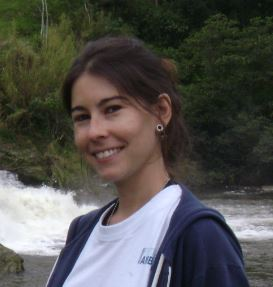
\includegraphics[width=0.15\textwidth]{figuras/helena}
\end{wrapfigure}
O mapeamento de solos enfrenta nos dias de hoje grandes desafios para atender a demanda da sociedade por informações em nível de detalhe adequado para o planejamento de uso da terra e dos recursos naturais. Paralelamente, a melhoria da capacidade de processamento dos computadores aliada a disponibilidade de programas e dados estruturados em ambiente de Sistemas de Informações Geográficas (SIG), impulsiona a utilização de novas ferramentas e métodos de análise aplicados aos estudos ambientais.\\
A formação de novos pedólogos vivência um momento emblemático, que pode ser considerado um hiato no contexto do levantamento de solos no país, onde se denota carência em transferência de conhecimentos e experiências práticas, agravada pela ausência de grandes projetos e incentivos governamentais para treinamento e capacitação deste tipo de profissional, diga-se de passagem, escasso no país.\\
Neste contexto, o ensino de ciências do solo reflete a necessidade de atualização e discussão de conceitos e métodos clássicos, considerando a inserção de ferramentas modernas de análise espacial buscando aperfeiçoar os procedimentos inerentes à atividade de levantamento, desde o planejamento amostral até a análise e apresentação dos dados obtidos. Não obstante, o uso de técnicas de Mapeamento Digital de Solos (MDS) confere um caráter quantitativo, com conhecimento das incertezas associadas aos produtos gerados, tendo como base procedimentos estatísticos reproduzíveis, conforme apresentado por \cite{CarvalhoJuniorEtAl:2011, ChagasEtAl:2011, CrivelentiEtAl:2009, GiassonEtAl:2006, WiesmeierEtAl:2010, tenCatenEtAl:2011}.\\
A oportunidade de participar de uma disciplina direcionada ao MDS motivou a elaboração deste artigo, que tem o objetivo principal de relatar a experiência como aluna de doutorado do Curso de Pós-Graduação em Agronomia -- Ciência do Solo (CPGA-CS, UFRRJ), membro integrante da Rede Brasileira de Pesquisa em Mapeamento Digital de Solos (RedeMDS) e da Comissão de Pedometria da Sociedade Brasileira de Ciência do Solo (Divisão 1.3.1 da SBCS).\\
Em primeira instância, encarei esta oportunidade como uma forma de contribuir para a discussão dos procedimentos intrínsecos ao levantamento de solos, relevantes para a formação de novos pedólogos e consequentemente, para a continuidade e prosperidade desta nobre profissão, restrita à experiência e conhecimento tácito de alguns profissionais, cada vez mais raros. Dito isso, escrevo este artigo para prestigiar a iniciativa de difusão do conhecimento nesta temática considerada pioneira no país, no que tange ao ensino e capacitação de novos pedólogos no uso de ferramentas modernas de análise espacial de dados e mapeamento digital.\\
A disciplina intitulada ``Métodos e Técnicas de Mapeamento Digital de Solos (Tópicos Especiais em Ciência do Solo-T.E.C.S.)'', oferecida no Curso de Pós-Graduação em Agronomia - Ciência do Solo (CPGA-CS), teve como público alvo estudantes de pós-graduação e professores da Universidade Federal Rural do Rio de Janeiro (UFRRJ).\\
De uma forma geral, as aulas ministradas abordaram o manuseio de dados primários e obtenção de secundários, treinamento com ferramentas de SIG e programas específicos, formas de aplicação e análise de modelos preditivos no mapeamento de classes e atributos dos solos.\\
O período de duração da disciplina coincidiu com a realização da 3º Reunião da RedeMDS e do 34º Congresso Brasileiro de Ciência do Solo (XXXVI CBCS), no mês de agosto na cidade de Florianópolis (SC) que promoveu o encontro de pesquisadores e estudantes para discussão de assuntos relacionados a esta temática.\\
Este conjunto de circunstâncias contou ainda com uma feliz coincidência que merece ser mencionada no contexto desta narrativa. Após o término dos eventos supracitados a UFRRJ recebeu a visita do pesquisador Philip Owens, Professor da Universidade de Purdue (Indiana - EUA). Tal fato oportuno ocorreu no período de aulas da disciplina, o que propiciou o contato e a troca de experiências com professor de instituição estrangeira de excelência no ensino de ciências agrárias, com potencial para construção de parceria e intercâmbio de estudantes e pesquisadores. Philip prestou contribuição à disciplina na forma de palestras, onde expôs parte das suas ideias e trabalhos relacionados ao emprego de MDS na hidropedologia, mostrando uma gama de possibilidades para aquisição de dados e de interpretação dos produtos derivados dos levantamentos de solos. E ainda, ressaltou que o uso destas técnicas tem em vista fornecer informações úteis e estratégicas para a sociedade que sirvam como subsídio para o planejamento de uso dos 
recursos naturais. Em suas explanações preconizou a aplicação destas técnicas na avaliação do potencial e das limitações das terras para produção agrícola entre outras atividades, destacando a importância do solo como organismo natural atuante na renovação (filtragem da água), recarga, conservação e manutenção de mananciais hídricos superficiais e sub-superficiais.\\
Sendo assim, a difusão de técnicas e capacitação de profissionais no uso das ferramentas e análise de dados em ambiente SIG, tem cunho estratégico e promissor contribuindo para o desenvolvimento científico e inovação tecnológica do país. Não obstante, as informações que podem ser extraído vão além da representação espacial de dados de solos, servido de base para estudos relacionados à prospecção mineral, dinâmica da água, potencial agrícola, aspectos geotécnicos, entre outras interpretações. Sob a ótica da taxonomia e classificação de solos é possível que a aplicação extensiva destas técnicas possa facilitar a identificação de fatores locais típicos para definição de classes em nível categórico de famílias e series, possibilitando o estudo da variabilidade das propriedades das distintas classes de solos e níveis categóricos.\\
Acredito em um ``futuro não muito distante'' onde a importância do MDS seja reconhecida e difundida através de criação de linha de pesquisa com enfoque em pedometria e mapeamento, com inserção de disciplinas regulares que abordem esta temática na formação de novos pedólogos. Sob um ponto de vista mais abrangente, ações desta natureza contribuem para melhor entendimento das relações solo-paisagem e aspectos do ambiente. Com o emprego extensivo de ferramentas e programas de geoprocessamento em estudos ambientais é plausível considerar que pesquisas estruturadas sob a perspectiva do MDS produzam ricos banco de dados georreferenciados e sistematizados, que são muito úteis para elaboração de modelos preditivos complexos e importantes para o planejamento de ocupação das terras e tomada de decisões relacionadas ao uso de recursos naturais.\\
Na primeira aula do curso foi indagado aos alunos quais as perspectivas individuais sobre a disciplina e as formas de aplicação das técnicas de MDS em seus respectivos estudos. Observei que inicialmente muitos dos participantes não imaginavam as possibilidades e diversidade de análises e interpretações dos produtos gerados. Este quadro se transformou com o passar das aulas, onde foi possível perceber o crescente interesse, através do surgimento de dúvidas e observações emitidas pelos participantes de forma direcionada às aplicações práticas do conhecimento adquirido.\\
Pessoalmente, tive a impressão que alguns dos participantes não tinham contato prévio com os softwares e técnicas utilizadas, sendo a familiarização com a linguagem e ambientação com os comandos e operações, construída gradativamente.\\
O treinamento preliminar em ferramentas e programas de geoprocessamento, e também o domínio dos conceitos de gênese de solos, modelos clássicos e padrões de ocorrência na paisagem e procedimentos do mapeamento, representaram fonte de complicação por parte de alguns alunos. Sendo assim, tais requisitos são desejáveis para melhor aproveitamento do conteúdo lecionado. Considero ainda, a subdivisão dos assuntos tratados na disciplina em dois âmbitos elementares, que podem ser objeto de módulos sequenciais. Um deles com caráter introdutório e abordagem teórica pode tratar dos conceitos básicos envolvidos na atividade de levantamento de solos, e procedimentos de pré-processamento e manuseio de dados espaciais georreferenciados, para obtenção das variáveis discriminantes e análise das co-relações solo-paisagem. O outro módulo tange ao treinamento em ferramentas de modelagem digital e algoritmos preditivos para o mapeamento digital de classes e atributos dos solos, incluindo a análise dos produtos do MDS, incertezas 
associadas e interpretações derivadas. O conteúdo deste módulo pode ser ministrado com base em um estudo de caso (dados reais), motivando a utilização destas técnicas em áreas de referência.\\
Diante do exposto, novamente parabenizo a concretização desta disciplina, que mesmo em caráter incipiente, como matéria de tópicos especiais oferecida para alunos pós-graduação, significa uma nova tendência no ensino de ciência de solo e inspira uma nova geração de pedólogos, com capacidade de compreensão e aplicação de conceitos clássicos e capacitação em ferramentas modernas de análise espacial, que possam contribuir com o aperfeiçoamento e retomada das atividades ligadas ao levantamento de solos no Brasil.\\
Cabe suscitar ainda, que a concretização do curso teve como precursora a existência da RedeMDS que promoveu a integração entre os pesquisadores deste ramo do conhecimento, o que inclui os responsáveis pela viabilização da disciplina e alguns alunos que utilizam MDS em seus estudos.\\
Enfim, espero que este relato sirva como incentivo e inspiração para estudantes, professores, técnicos, pesquisadores e instituições ligadas ao ensino de ciência do solo e capacitação de recursos humanos, para a difusão do conhecimento, possibilidades e limitações do uso de ferramentas de mapeamento digital aplicadas a levantamentos pedológicos.
\begin{footnotesize}
\begin{thebibliography}{99}
\bibitem[Carvalho Júnior et~al. (2003) Carvalho Júnior, Chagas, Fernandes, Vieira, Schaefer, Bhering, Francelino]{CarvalhoJuniorEtAl:2011}
W. de Carvalho Júnior, C. da S. Chagas, E.I. Fernandes, C.E. Vieira, C.E.G. Schaefer, S.B. Bhering, M.R. Francelino (2011)
\newblock Digital soilscape mapping of tropical hillslope areas by neural networks.
\newblock {\em Scientia Agricola} 68: 691-696.
\bibitem[Chagas et~al. (2011) Chagas, Carvalho Júnior, Bhering]{ChagasEtAl:2011}
C. de S. Chagas, W. de Carvalho Júnior, S.B. Bhering (2011)
\newblock Integração de dados do Quickbird e atributos do terreno no mapeamento digital de solos por redes neurais artificiais.
\newblock {\em R. Bras. Ci. Solo} 35: 693-704.
\bibitem[Crivelenti et~al. (2009) Crivelenti, Coelho, Adami, Oliveira]{CrivelentiEtAl:2009}
R.C. Crivelenti, R.M. Coelho, S.F. Adami, S.R. de M. Oliveira (2009)
\newblock Mineração de dados para a inferência de relações solo-paisagem em mapeamentos digitais de solo.
\newblock {\em Rev. Agro. Bras.} 44: 1707-1715.
\bibitem[Giasson et~al. (2006) Giasson, Clarke, Inda Junior, Merten, Tornquist]{GiassonEtAl:2006}
E. Giasson, R.T. Clarke, A.V. Inda Junior, G.H. Merten, C.G. Tornquist (2006)
\newblock Digital soil mapping using multiple logistic regression on terrain parameters in southern Brazil.
\newblock {\em Sci. Agric.} 63: 262-268.
\bibitem[ten Caten et~al. (2011) ten Caten, Dalmolin, Pedron, Mendonça-Santos]{tenCatenEtAl:2011}
A. ten Caten, R.S.D. Dalmolin, F.A. Pedron, M.L. Mendonça-Santos (2011)
\newblock Extrapolação das relações solo-paisagem a partir de uma área de referência.
\newblock {\em Ci. Rural.} 41: 812-816.
\bibitem[Wiesmeier et~al. (2010) Wiesmeier, Barthold, Blank,  Kögel-Knabner]{WiesmeierEtAl:2010}
M. Wiesmeier, F. Barthold, B. Blank,  I. Kögel-Knabner (2010)
\newblock Digital mapping of soil organic matter stocks using Random Forest modeling in a emi-arid steppe ecosystem.
\newblock {\em Plant Soil} 340: 7-24.
\end{thebibliography}
\end{footnotesize}
\address{Helena Saraiva Koenow Pinheiro\\
  Universidade Federal Rural do Rio de Janeiro\\
  \email{lenask@gmail.com}}
\end{article}

\begin{article}
   \title{Uso de técnicas baseadas no conhecimento e lógicas \emph{fuzzy}}
\subtitle{Predição de classes e atributos de solos}
\author{por Michele Duarte de Menezes}
\maketitle
\begin{wrapfigure}{l}{0.15\textwidth}
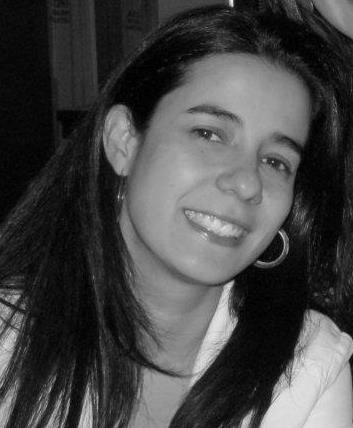
\includegraphics[width=0.15\textwidth]{figuras/foto-michele.png}
\end{wrapfigure}
Atualmente, diversas técnicas têm sido usadas para a predição de solos e seus atributos, algumas com a promessa de aumentar a acurácia, reduzir os custos e o tempo de execução. De um lado, temos as técnicas mais quantitativas ou pedométricas, onde a predição é baseada em técnicas estatísticas, geoestatísticas, mineração de dados ou de aprendizado de máquinas, e que, de modo geral, requerem um esquema amostral mais denso. Do outro lado, as técnicas baseadas no conhecimento, que buscam empregar efetivamente o conhecimento tácito (informações e técnicas adquiridas por experiência) na predição, com o intuito de reduzir algumas inconsistências e o custo dos mapeamentos manualmente confeccionados. Contudo, as técnicas pedométricas e as baseadas no conhecimento não são mutuamente exclusivas, e para ambas, o conhecimento das relações de solo-paisagem e prospecções de campo são necessários.\\
Hudson (1992), em seu consagrado artigo \emph{Soil Survey as Paradigm-based Science}, levantou que a maior parte do conhecimento a respeito de solos e paisagens encontra-se na forma de mapas de solos. Tal conhecimento, portanto, não é totalmente explícito aos demais usuários. E ainda, conforme levantado pelo Prof. Marcos Bacis Ceddia (UFRRJ) em sua palestra no Congresso Brasileiro de Ciência do Solo (2013), que abordou a respeito do mapeamento digital de solos - ou, conforme suas palavras, o mapeamento de solos no nosso tempo - se Dokuchaev estivesse vivo, quais ferramentas ele utilizaria para mapeamento? Será que o conhecimento já obtido, tanto tácito como em forma de mapas seriam ignorados?\\
Diante de tais técnicas, apontamentos e questões, apresento-lhes dois \emph{softwares} que fornecem um conjunto de ferramentas aos pedólogos para formalizarem as relações de solo-paisagem a partir de seus conhecimentos, de um modo mais quantitativo. O SoLIM (\emph{Soil Land Inference Model}) e o ArcSIE (\emph{Soil Inference Engine}) foram criados com o intuito de melhorar os métodos, a eficiência e a acurácia dos mapeamentos. O SoLIM é um software livre, já o ArcSIE é uma extensão do ArcGIS, mas é possível fazer o seu download gratuitamente. Tais ferramentas empregam alguns componentes, como o conhecimento especialista (\emph{expert}), a lógica \emph{fuzzy} ou nebulosa e vetores de similaridade.\\
Sistemas de conhecimento \emph{expert} buscam capturar o conhecimento tácito e integrá-lo em modelos de predição. Já a lógica \emph{fuzzy} configura-se como uma alternativa à lógica Booleana (modelo discreto, mapa do tipo polígono) no processo de inferência. A transição entre solos na paisagem se dá, frequentemente, de modo mais gradual e contínua, diferentemente das variações representadas por um mapa de polígono (Booleano). Existe certa incerteza na alocação dos limites entre os solos. Nesse sentido, a lógica \emph{fuzzy} busca representar a incerteza na predição, aplicando conceitos de verdade parcial, uma alternativa a rigidez subjetiva imposta aos solos.\\
Trazendo esses conceitos para uma aplicação mais real, a partir de covariáveis ambientais que representam os fatores de formação do solo em base SIG, e o ajuste de curvas de pertinência \emph{fuzzy}, as seguintes relações podem ser formalmente estabelecidas: em uma dada região fisiográfica, sabe-se que os Neossolos Litólicos ocorrem em faixas de altitude maiores que 850 m, cujo relevo é escarpado, a forma das vertentes são predominantemente côncavas e são formados a partir de granito-gnaisse. Uma vez que existe o conhecimento detalhado sobre as relações de solo paisagem da região, estabelecem-se curvas de pertinência \emph{fuzzy} para cada uma dessas instâncias, que consistem na base para a criação de mapas de pertinência \emph{fuzzy}. Um exemplo é dado para a declividade na \ref{fig:figura1}.\\
O conceito de pertinência ou pertencer a um grupo é modificado para incluir graus parciais de pertinência. O valor máximo de pertinência é geralmente 1 e representa o centro ou o conceito modal, e 0 representa não-pertinência (representados no eixo Y do gráfico). Valores entre 0 e 1 expressam diferentes graus de similaridade para o conceito central do tipo de solo. Conforme a curva ajustada (Figura 1), quanto maior a declividade (eixo X), maior o valor de pertinência (mais próximo de 1). Mais especificamente para o Neossolo Litólico e a declividade, ajusta-se o valor de 75 para o \emph{low unity} (relevo escapado apresenta declives maiores que 75\%, o que representa o valor ideal para ocorrência de Neossolos Litólicos, com valores de pertinência aumentando conforme aumenta a declividade), ajusta-se o valor de 45\% para o \emph{low cross} (valor que representa 50\% de pertinência \emph{fuzzy}).\\
\begin{figure*}[tb!]
\begin{minipage}[t]{1\linewidth}
\begin{center}
 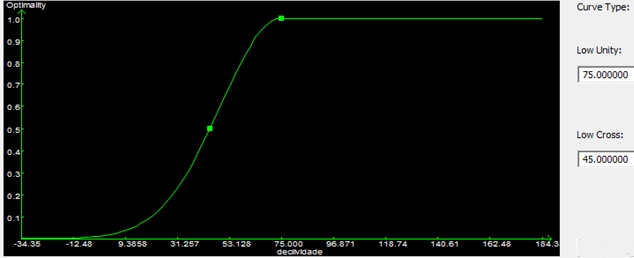
\includegraphics[width=\textwidth]{figuras/figura1.png}
 \caption{\emph{Layout} do SoLIM para o ajuste de curvas de pertinência \emph{fuzzy}.}
 \label{fig:figura1}
\end{center}
\end{minipage}
\end{figure*}
O próximo passo consiste na geração do mapa de pertinência \emph{fuzzy} a partir da curva gerada para a declividade, conforme apresentado na \ref{fig:figura2}. Quanto mais similar o solo ao conceito central prescrito, maior o valor de pertinência \emph{fuzzy} (mais próximo a 100). Estes conceitos são aplicados pixel a pixel. Notem a natureza contínua da distribuição, que serão a base para a composição do mapa de solos (polígono) e atributos (contínuo). Curvas devem ser ajustadas para as outras covariáveis, contemplando todas as instâncias e as diferentes classes de solos da área.\\
\begin{figure*}[tb!]
\begin{minipage}[t]{1\linewidth}
\begin{center}
   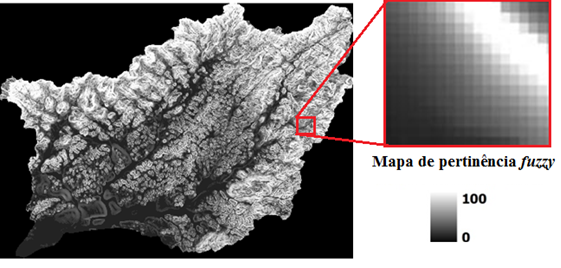
\includegraphics[width=\textwidth]{figuras/figura2.png}
   \caption{Mapa de pertinência \emph{fuzzy} gerado a partir do mapa de declividade.}
   \label{fig:figura2}
\end{center}
\end{minipage}
\end{figure*}
Para criar o mapa do tipo polígono, o ArcSIE ou SoLIM classificam pixel a pixel com o valor mais elevado de pertinência \emph{fuzzy}, de acordo com vetores de similaridade. Conforme, a \ref{fig:figura3}, o pixel assinalado será classificado como Neossolo Litólico. Portanto, os valores de pertinência \emph{fuzzy} foram usados para medir a incerteza associada ao processo de ``endurecimento'' (\emph{hardened}) ou defuzzificação do solo local, para gerar o mapa do tipo polígono.\\
E ainda, a partir das curvas estabelecidas e os mapas de pertinência \emph{fuzzy}, é possível a predição de atributos do solo de modo mais contínuo, a partir de apenas um valor típico, ou seja, um valor que melhor represente o conceito central ou modal de cada tipo de solo para a sua predição píxel a píxel na paisagem.\\
Eu comentei aqui apenas alguns pontos chave do processo de inferência. Detalhes sobre a matemática, os tipos de curvas ajustadas, bem como a estruturação das instâncias podem ser encontradas nos tutoriais dos softwares. Tanto o ajuste de curvas como a escolha dos valores típicos, tornam explícitos todos os detalhes da modelagem de solos e atributos, tornando-os assim potencialmente aplicáveis para outras regiões cujas relações de solo-paisagem são semelhantes. Acredito que seja esse um dos motivos para os autores considerarem tais ferramentas como promissoras para o mapeamento em massa, de modo mais rápido e com um menor custo.\\
\begin{figure}[htbp]
   \centering
   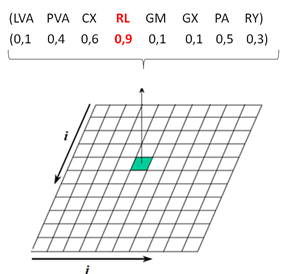
\includegraphics[scale=0.8]{figuras/figura3.png}
   \caption{Figure 3. Modelos de similaridade para representar informação espacial de solos.}
   \label{fig:figura3}
\end{figure}
Outra ferramenta interessante é o \emph{knowledge miner} (mineração do conhecimento), presente no SoLIM. Sob a premissa de que os mapas de solo representam a estrutura mental do pedólogo a respeito das relações de solo-paisagem, o usuário pode extrair informações de mapas pré-existentes por meio de curvas de frequência relativa, a partir de mapas derivados do terreno para cada polígono ou unidades de mapeamento. São computadas distribuições univariadas baseadas na estimação não-paramétrica de kernel. As curvas de frequência permitem descobrir o conhecimento \emph{expert} empregado. Nos Estados Unidos, esta ferramenta tem sido empregada para atualizar os mapas de solos já existentes, permitindo também detectar inconsistências. No Brasil, uma potencial aplicação desta ferramenta está na extração das curvas de frequência relativa em áreas de referência que possuem levantamentos de solos, e sua transferência para outras sem levantamento, mas com similaridade em termos de fatores de formação dos solos. 
Levantamentos de solos em escalas mais detalhadas são ainda necessários. Eis uma ferramenta promissora para aumentar a expressão geográfica de áreas mapeadas, com um menor custo.\\
Conforme levantado por alguns dos criadores do SoLIM (Shi et al., 2009 - \emph{Integrating Different Types of Knowledge for Digital Soil Mapping}), a aceitação de uma ferramenta é de suma importância: o usuário deve acreditar no sistema, e esta confiança é geralmente baseada no entendimento do usuário sobre o sistema. Os autores apontam também para uma maior aceitação desta ferramenta por parte dos pedólogos devido ao fato da abordagem ser baseada no conhecimento. De fato, tenho percebido também uma boa aceitação entre os mapeadores de solos os quais já comentei ou foram apresentados a ferramenta.\\
Pessoalmente, tive oportunidade de utilizar tais ferramentas durante o meu doutorado. Fui orientada pelo Prof. Nilton Curi (UFLA), um grande pedólogo que possui vasto conhecimento das relações de solo-paisagem das regiões em que desenvolvemos trabalhos. Fui orientada também pelo Prof. Phillip Owens (\emph{Purdue University}), cuja linha de pesquisa está um pouco mais relacionada ao mapeamento digital. A integração de tais conhecimentos, bem como o uso das ferramentas, me permitiu compreender, sedimentar e formalizar as relações de solo-paisagem de um modo mais quantitativo. Durante este período, lembrei-me de quando estava aprendendo a ler em minha infância. Para mim, era inevitável ler tudo ao meu redor a todo tempo: anúncios pelas ruas, jornais, revistas, televisão, etc. Do mesmo modo, quando comecei a aprender um pouco mais sobre a lógica \emph{fuzzy}, foi inevitável tentar ``encaixar'' ou ``ler'' os solos e outros fenômenos da natureza sob a ótica da lógica \emph{fuzzy}.\\
Já com relação às ferramentas propriamente ditas, quando comecei a usá-las faltavam alguns detalhes nos tutoriais, o que me fez gastar um tempo elevado com pequenos detalhes durante a modelagem. No entanto, os tutoriais foram muito melhorados desde então, e muitos artigos já foram publicados. Contudo, acho que o aprendizado da modelagem de solos por meio do ArcSIE ou SoLIM chega até ser um pouco intuitivo, o que é mais ou menos semelhante ao processo de mapeamento de solos.\\
O grande desafio, principalmente para esta técnica embasada no conhecimento, está na leitura da paisagem, no resgate da Geomorfologia, na aplicação adequada da Geomorfometria, e o afinamento com os conceitos da Pedologia. Isso se faz necessário pois os mapas de hoje requerem não apenas um \emph{layout} bonito, com cores atrativas, mas uma acurácia adequada, com a quantificação das incertezas, e geração de produtos para atender efetivamente as necessidades da sociedade. As atividades de campo são cruciais. Atrelar estas ferramentas à técnicas de mineração de dados podem ainda trazer informações relevantes à modelagem.\\
Existem ainda muitas áreas a serem mapeadas, e muito a ser testado com relação as ferramentas. Encorajo os interessados em mapeamento digital a aventurarem-se pelos tutoriais gratuitamente disponíveis na internet, que contém ainda uma base de dados para uma primeira familiarização.\\
\\
Link dos softwares para donwload:\\
SoLIM: \url{http://solim.geography.wisc.edu/about/index.htm}\\
ArcSIE: \url{http://www.arcsie.com/}\\
\\
\address{Michele Duarte de Menezes\\
  Universidade Federal Rural do Rio de Janeiro\\
  \email{michele\_duarte@ig.com.br}}

%%% Local Variables: 
%%% mode: latex
%%% TeX-master: documento-principal.tex
%%% End: 


\end{article}

\begin{article}
   \title{Assinatura geomorfométrica: potencial para estudos pedométricos}
\author{por Vinicius Vasconcelos}
\maketitle
\begin{wrapfigure}{l}{0.15\textwidth}
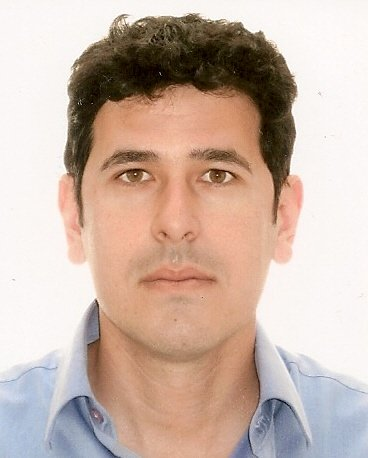
\includegraphics[width=0.15\textwidth]{figuras/foto-vini.jpg}
\end{wrapfigure}
Muitos estudos têm sido realizados para obter uma descrição detalhada das formas de terreno com o propósito de compreender a evolução da paisagem. Nesta perspectiva, consolida-se o campo da ciência denominada de \emph{(Geo)morfometria} que analisa a superfície topográfica de forma quantitativa. Esta disciplina também é conhecida como \emph{análise de terreno} ou \emph{modelagem digital de terreno} \citep{LaneEtAl1998, Pike:2000}.\\
Um dos pressupostos levantados pela Geomorfometria é a obtenção das feições do relevo de maneira automática ou semi-automática.  É importante citar alguns trabalhos dentro dessa perspectiva. Eu começaria por \cite{Wood:1996}, uma tese de doutorado disponível no endereço \url{http://www.soi.city.ac.uk/~jwo/phd/}. O autor obteve seis feições morfométrica conhecidas como \emph{peak}, \emph{pass}, \emph{channel}, \emph{pit}, \emph{plane} e \emph{ridge} a partir de curvaturas, vertical, longitudinal, transversal, mínima e máxima.  O método considera uma combinação específica dos pares de curvaturas Longitudinal/Transversal e Mínima/Máxima a depender da declividade da região a ser classificada. Assim, as curvaturas Longitudinal/Transversal são apenas utilizadas quando o relevo apresenta uma declividade mais acentuada. Consequentemente, as curvaturas e Mínima e Máxima são utilizadas em áreas de relevo mais suave. Desta forma, a combinação das curvaturas apresenta uma relação excludente de acordo com o relevo que 
será modelado.\\
A observação das curvaturas como parâmetro da análise na identificação do tipo de solo é muito antiga.  \cite{Aandahl:1948} foi o primeiro a reconhecer a influência das curvaturas de plano e de perfil na formação e distribuição dos solos. \cite{Troeh:1964} desenvolveu o primeiro método quantitativo para estimar curvaturas horizontais e verticais e relacioná-los com as propriedades dos solos. \cite{Pennock:1987} em seguida definiu, por meio das curvaturas verticais e horizontais, uma combinação das primeiras Formas de Terreno (FT) ou \emph{landforms} para estudo de solos.\\
O trabalho que está em desenvolvimento no Laboratório de Sistema de Informações Espaciais (LSIE) do Departamento de Geografia da Universidade de Brasília - UnB, tem como perspectiva compreender melhor a evolução do relevo a partir dos atributos pedológicos a partir técnicas de classificação de Formas de Terreno. O nosso trabalho mais recente é na elaboração de uma curva que possa explicar as variações da intensidade do relevo.\\
Nesse estudo utilizamos dados de curvatura: Vertical, Longitudinal, Transversal, Mínimo, Máximo e Horizontal organizados em uma só imagem com bandas de curvatura com consequente formação de uma  assinatura geomorfométrica \citep{Vasconcelos:2012}. Esta assinatura consiste na formulação de uma curva das medidas topográficas capaz de distinguir as diferentes paisagens. Assim, cada célula da grade (unidade de terreno) é descrita por uma curva dos atributos de terreno que pode ser comparada com curvas específicas de formas de relevo (assinaturas). Esta abordagem conduz ao emprego de técnicas de reconhecimento de padrões a partir de métodos estatísticos multivariados comumente empregados no processamento digital de imagens de sensoriamento remoto \citep{BrownEtAl:1998}.\\
Primeiramente é utilizado o método Menor Fração de Ruído (MFR). Esse método funciona como uma Análise de Principal Componente, determina a dimensionalidade inerente dos dados de imagem, para separar o ruído nos dados, e reduzir os requisitos de cálculo para um processamento subsequente \citep{BoardmanEtAl:1994}. Em uma imagem composta por curvaturas, o MFR vai selecionar as informações que mais se repetem na imagem. Em seguida, utiliza-se outro método para por fim identificar as assinaturas geomorfométricas: Indice de Pureza do Pixel. Esse processamento foi desenhado para localizar os mais extremos (valor único ou diferente ou "puro"), pixels \citep{BoardmanEtAl:1995}. Os pixels mais puros tipicamente correspondem a um membro final, ou seja, uma curva padrão de forma de terreno.\\
O método de assinatura geomorfométrica reconhece não só o padrão de uma Forma de Terreno, mas também a sua intensidade, permitindo identificar e classificar inúmeras formas. Nesse sentido, esse procedimento pode auxiliar na escolha de áreas de referência para estudos pedológicos assim como na relação solo-paisagem.
\begin{footnotesize}
\begin{thebibliography}{99}
\bibitem[Boardman et~al. (1994) Boardman, Kruse]{BoardmanEtAl:1994}
J.W. Boardman, F.A. Kruse (1994)
\newblock Automated  spectral analysis a geological example using AVIRIS data, North Grapevine, Mountains, Nevada.
\newblock {\em Proceedings of the Tenth Thematic Conference on Geological Remote Sensing, San Antonio} pp.407-418.
\bibitem[Boardman et~al. (1995) Boardman, Kruse, Green]{BoardmanEtAl:1995}
J.W. Boardman, F.A. Kruse, R.O. Green (1995)
\newblock Mapping target signatures via partial unmixing of AVIRIS data
\newblock {\em Annual JPL Airborne Geosciences Workshop, Pasadena} pp.23-26.
\bibitem[Brown et~al. (1998) Brown, Lusch, Duda]{BrownEtAl:1998}
D.G. Brown, D.P. Lusch, K.A. Duda (1998)
\newblock Supervised classification of glaciated landscape types using digital elevation data.
\newblock {\em Geomorphology} 21: 233-250.
\bibitem[Lane et~al. (1998) Lane, Richards, Chandler]{LaneEtAl1998}
S.N. Lane, K.S. Richards, J.H. Chandler (1998)
\newblock Landform Monitoring, Modelling and Analysis.
\newblock {\em Wiley} 466 pp.
\bibitem[Jo Wood (1996)]{Wood:1996}
J. Wood (1996)
\newblock The  Geomorphological  Characterisation of Digital Elevation Models.
\newblock {\em Thesis (PhD in Science Information)} 184p.
\bibitem[Aandahl (1948)]{Aandahl:1948}
A.R. Aandahl (1948)
\newblock The characterization of slope positions and their influence on the total N content of a few virgin soils in Western Iowa.
\newblock {\em Soil Science Society of America Journal} 13: 449–454.
\bibitem[Troeh (1964)]{Troeh:1964}
F.R. Troeh (1964)
\newblock Landform parameters correlated to soil drainage.
\newblock {\em Soil Science Society of America Journal} 28: 808–812.
\bibitem[Pennock et~al. (1987) Pennock, Zebarth, De Jong]{Pennock:1987}
D.J. Pennock, B.J. Zebarth, E. De Jong (1987)
\newblock Landform  Classification  and  Soil Distribution in Hummocky Terrain, Saskatchewan, Canada.
\newblock {\em Geoderma} 40: 297-315.
\bibitem[Pike (2000) Pike]{Pike:2000}
R.J. Pike (2000)
\newblock Geomorphometry — diversity in quantitative surface analysis.
\newblock {\em Progress in Physical Geography} 24: 1-20.
\bibitem[Vasconcelos et~al. (2012) Vasconcelos, Carvalho Junior, Martins, Guimarães, Gomes]{Vasconcelos:2012}
V. Vasconcelos, O.A. Carvalho Junior, E.S. Martins, A.F. Couto Junior, R.F. Guimarães, R.A.T. Gomes (2012)
\newblock Sistema de Classificação Geomorfométrica baseado em uma arquitetura sequencial em duas etapas: Árvore de Decisão e Classificador Espectral, no Parque Nacional da Serra da Canastra.
\newblock {\em Revista Brasileira de Geomorfologia} 13: 171-186.
\end{thebibliography}
\end{footnotesize}
\address{Vinicius Vasconcelos\\
  Universidade de Brasília\\
  \email{vinicius.vascoza@gmail.com}}
%%% Local Variables: 
%%% mode: latex
%%% TeX-master: documento-principal.tex
%%% End:
\end{article}

\newpage

\begin{article}
   \title{Um pouco de R na \textit{Newsletter}}
\subtitle{Nuvem de palavras}
\author{por Alessandro Samuel-Rosa}
\maketitle
\begin{wrapfigure}{l}{0.15\textwidth}
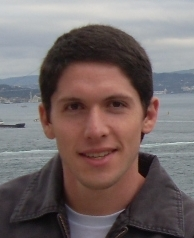
\includegraphics[width=0.15\textwidth]{figuras/foto-alessandro}
\end{wrapfigure}
O ambiente de análise de dados \R{} possui uma imensidade de funcionalidades que vão desde simples operações algébricas até a modelagem de complexas relações entre o solo e os fatores de formação do solo. Um bom exemplo do último caso é mostrado acima no artigo do Waldir, do Cesar e da Michele sobre a disciplina de mapeamento digital de solos ministrada na Universidade Federal Rural do Rio de Janeiro. Mas o que poucos sabem é que, sendo um ambiente de análise de dados, e não um simples software estatístico, quaisquer tipos de dados podem ser analisados no \R{}. Isso inclui dados contínuos, categóricos, imagens, vetores, volumes, 1D, 2D, 3D, 4D, áudio, vídeo, texto, e mais uma infinidade de possibilidades. Mas hoje vou me deter à apenas um destes tipos de dados, os dados textuais.
\subsection{Nuvem de palavras}
No presente número da \textit{Newsletter} da Comissão de Pedometria, uma novidade foi apresentada na página de abertura: um logo formado por uma nuvem de palavras.\\
\\
\emph{Uma nuvem de palavras, ou nuvem de tags, é uma representação visual de dados textuais onde a importância de cada palavra no texto é mostrada com o tamanho da fonte ou cor} \citep{wiki:2013}.\\
\\
Os dados textuais utilizados aqui são representados pelo conteúdo do seguinte vetor:
\begin{smallverbatim}
 > words <- c("pedometria pedometria pedometria
 pedometria solo estatística matemática sensores
 pedologia mapeamento gênese espaço variabilidade
 amostra dados métodos variação informática
 tecnologia programação script amostragem GPS
 satélite MDE pedólogo regressão geoestatística
 pedotransferência modelos resíduo incerteza
 computador mapas covariáveis tempo 3D função
 validação calibração SIG sistema predição
 interpolação ajuste curva rede neural árvore
 decisão classificação especialista erro
 correlação seleção automático paisagem logística
 simulação terreno atributo geologia clima imagem
 pixel escala resolução ensino pesquisa extensão
 agricultura ambiente precisão acurácia")
\end{smallverbatim}
A composição do vetor de dados textuais foi definida a partir da minha memória dos termos mais relacionados à pedometria. Como minha memória é falha e enviesada pelas minhas experiências pessoais, é provável que muitos outros termos poderiam ter sido incluídos. Sugestões são bem vindas para preparar o logo dos próximos números da \textit{Newsletter}. Além disso, outros dados textuais também podem ser analisados, como por exemplo o conteúdo textual de um artigo, livro ou até mesmo da \textit{Newsletter}. Como fazer isto é o que eu mostro abaixo.
\subsection{Instalando os pacotes necessários}
\label{subsec:pacotes}
Os pacotes necessários para a elaboração de uma nuvem de palavras, como aquela usada como logo da \textit{Newsletter}, são quatro: \texttt{wordcloud} \citep{Fellows:2013}, \texttt{tm} \citep{FeinererEtAl:2013}, \texttt{slam} \citep{HornikEtAl:2013}, e \texttt{RColorBrewer} \citep{Neuwirth:2011}. O pacote \texttt{wordcloud} é aquele que gera a nuvem de palavras usado como logo da \textit{Newsletter}. Já os pacotes \texttt{tm} e \texttt{slam} são dependências do pacote \texttt{wordcloud} usados na análise dos dados para a geração da nuvem de palavras. Para instalar e carregar estes pacotes basta usar os comandos:
\begin{smallverbatim}
> install.packages(c("wordcloud","tm", "slam",
"RColorBrewer"),
> repos = "http://cran.r-project.org")
> require(wordcloud)
> require(RColorBrewer)
\end{smallverbatim}
\subsection{Definindo a paleta de cores}
Depois de instalados e carregados os pacotes, define-se a paleta de cores usando o pacote \texttt{RColorBrewer}. São diversas as opções de paletas de cores do pacote \texttt{RColorBrewer}, cuja demonstração está além do objetivo deste artigo. Maiores informações podem ser encontradas acessando o endereço \url{http://colorbrewer2.org/}. No caso da nuvem de palavras usada como logo da \textit{Newsletter}, a paleta usada foi aquela identificada como \texttt{YlOrBr}, que varia entre as cores amarelo (\emph{yellow}), laranja (\emph{orange}) e marrom (\emph{brown}). O comando usado é o seguinte:
\begin{smallverbatim}
> pal <- brewer.pal(n = 9, name = "YlOrBr")
\end{smallverbatim}
\subsection{Gerando a nuvem de palavras}
Carregados os pacotes necessários, definidos os dados textuais e a paleta de cores, agora é possível invocar a função \texttt{wordcloud} para gerar a nuvem de palavras:
\begin{smallverbatim}
> wordcloud(words = words, min.freq = Inf,
random.order = FALSE, random.color = TRUE,
colors = pal, rot.per = 0.2, fixed.asp = TRUE)
\end{smallverbatim}
Os parâmetros fornecidos ao comando \texttt{wordcloud} definem o objeto do \R{} contendo os dados textuais (\texttt{words = words}), não havendo limite de frequência mínima para que um termo que aparece nos dados textuais seja apresentado graficamente (\texttt{min.freq = Inf}). Os termos são apresentados no gráfico em ordem decrescente de frequência (\texttt{random.order = FALSE}) e as cores da paleta (colors = pal) são atribuídas aleatoriamente (\texttt{random.color = TRUE}). Apenas 20\% dos termos podem ser apresentados graficamente na vertical (\texttt{rot.per = 0.2}), dando-se preferência pela apresentação gráfica com a relação de aspecto dos eixos x e y fixa (\texttt{fixed.asp = TRUE}).
\subsection{Salvando a nuvem de palavras como figura}
Depois de gerada a nuvem de palavras, existem diversas maneiras de salvar uma figura para usar, por exemplo, no cabeçalho da \textit{Newsletter}. A primeira opção é salvar um arquivo no formato *.pdf usando o seguinte comando:
\begin{smallverbatim}
> pdf(file = "wordcloud.pdf")
> wordcloud(words = words, min.freq = Inf,
random.order = FALSE, random.color = TRUE,
colors = pal, rot.per = 0.2, fixed.asp = TRUE)
> dev.off()
\end{smallverbatim}
A segunda opção é salvar um arquivo no formato *.png usando o seguinte comando:
\begin{smallverbatim}
> x11(width = 17/2.5, height = 7.5/2.5,
bg = "black")
> wordcloud(words = words, min.freq = Inf,
random.order = FALSE, random.color = TRUE,
colors = pal, rot.per = 0, fixed.asp = FALSE)
> savePlot(filename = "wordcloud-black.png")
> dev.off()
\end{smallverbatim}
Note que o arquivo salvo no formato *.png possui algumas peculiaridades, como por exemplo o uso do comando \texttt{x11()} para definir uma região de apresentação gráfica com $17/2.5$ polegadas de largura e $7.5/2.5$ polegadas de altura, com plano de fundo preto (\texttt{bg = "black"}). Além disso, nenhum termo foi permitido aparecer na vertical e a relação de aspecto dos eixos x e y foi mantida livre (\texttt{rot.per = 0} e \texttt{fixed.asp = FALSE}). Os produtos gráficos são mostrados pelas figuras \ref{fig:wordcloud} e \ref{fig:wordcloud-black}.\\
\\
\begin{figure}[htbp]
   \centering
   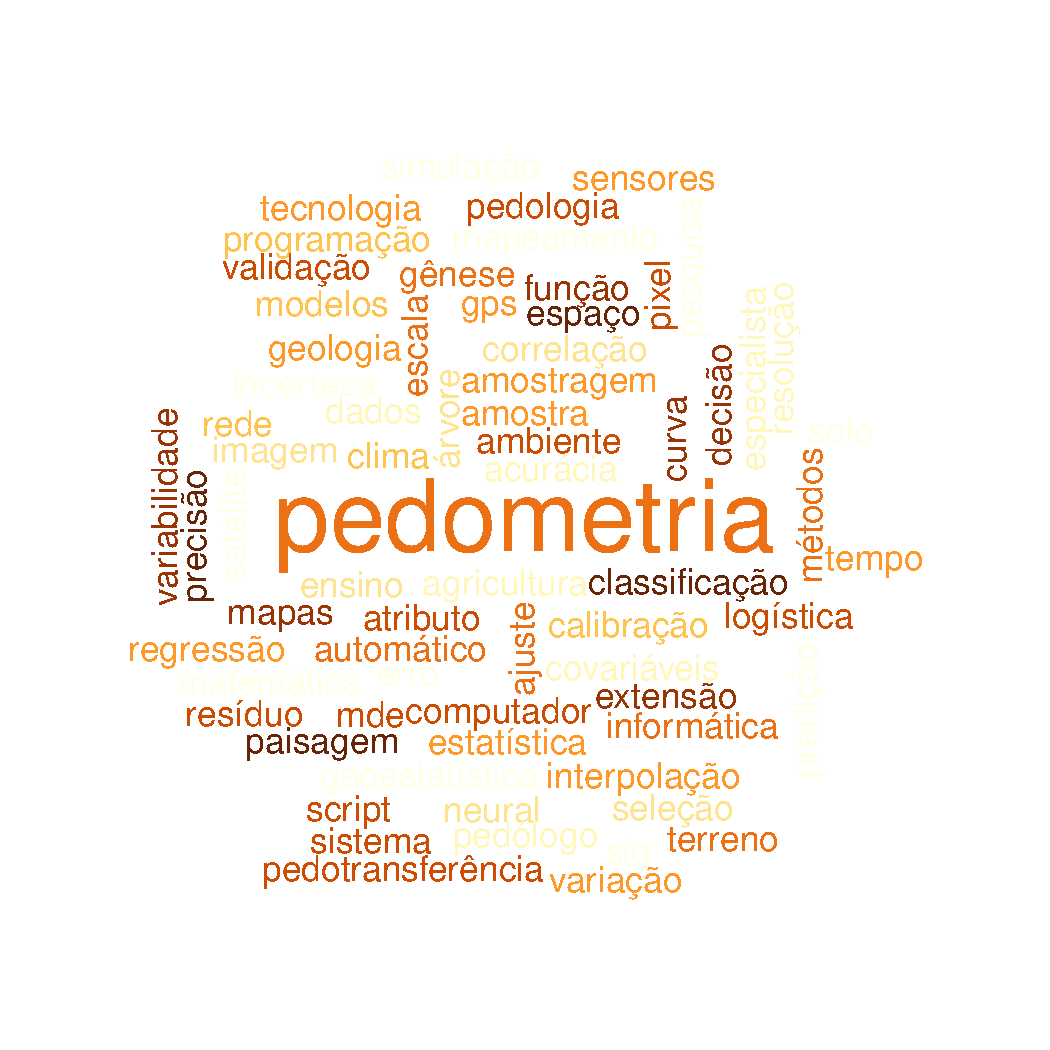
\includegraphics[scale=0.8]{figuras/wordcloud}
   \caption{Nuvem de palavras ligadas à pedometria com fundo branco e relação de aspecto fixa.}
   \label{fig:wordcloud}
\end{figure}
\noindent Diversas alterações podem ser feitas no produto gráfico final simplesmente alterando o conteúdo do vetor de dados textuais. Para aumentar ainda mais o tamanho do termo ``pedometria'' em relação aos demais termos, basta repeti-lo mais algumas vezes. Da mesma forma, se quisermos dar ênfase a outros termos, como por exemplo ``matemática'' e ``estatística'', basta repeti-los mais algumas vezes.\\
\\
\begin{figure}[htbp]
   \centering
   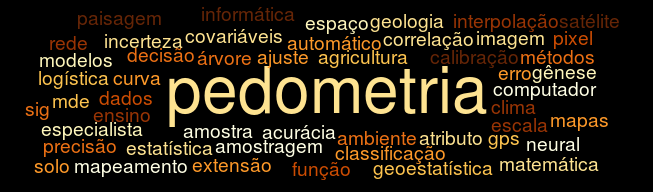
\includegraphics[scale=0.8]{figuras/wordcloud-black}
   \caption{Nuvem de palavras ligadas à pedometria com fundo preto e relação de aspecto livre.}
   \label{fig:wordcloud-black}
\end{figure}
\subsection{Um pouco de \R{} na \textit{Newsletter}}
Como eu disse no início deste artigo, existem diversos termos que poderiam ter sido acrescentados ao meu objeto contendo os dados textuais. Tais termos não foram incluídos simplesmente porque eu não lembrei deles ou porque não fazem parte do conjunto de termos que costumo relacionar à pedometria. É por este motivo que aqueles que gostarem de ver outros termos na nuvem de palavras que compõe o logo da \textit{Newsletter}, por favor, não exitem em entrar em contato pelo endereço de e-mail \email{alessandrosamuel@yahoo.com.br}. Ao mais aventureiros, o script usado no \R{} para produzir a nuvem de palavras pode ser baixado \href{http://goo.gl/tqGmI1}{clicando aqui} e usado para gerar novas e diferentes nuvens de palavras.
\begin{footnotesize}
\begin{thebibliography}{99}
\bibitem[Wikipedia (2013) Wikipedia]{wiki:2013}
Wikipedia (2013)
\newblock Tag cloud --- Wikipedia, The Free Encyclopedia.
\newblock \url{http://en.wikipedia.org/w/index.php?title=Tag_cloud&oldid=571203887} [Online; accessed 8-October-2013].
\bibitem[Fellows (2013) Fellows]{Fellows:2013}
I. Fellows (2013)
\newblock wordcloud: Word Clouds.
\newblock \url{http://CRAN.R-project.org/package=wordcloud} [R package version 2.4]
\bibitem[Feinerer \& Hornik (2013) Feinerer \& Hornik]{FeinererEtAl:2013}
I. Feinerer \& K. Hornik (2013)
\newblock tm: Text Mining Package.
\newblock \url{http://CRAN.R-project.org/package=tm} [R package version 0.5-9.1]
\bibitem[Hornik et~al. (2013) Hornik, Meyer \& Buchta]{HornikEtAl:2013}
K. Hornik, D. Meyer \& C. Buchta (2013)
\newblock slam: Sparse Lightweight Arrays and Matrices.
\newblock \url{http://CRAN.R-project.org/package=slam} [R package version 0.1-30]
\bibitem[Neuwirth (2011) Neuwirth]{Neuwirth:2011}
E. Neuwirth (2011)
\newblock RColorBrewer: ColorBrewer palettes.
\newblock \url{http://CRAN.R-project.org/package=RColorBrewer} [R package version 1.0-5]
\end{thebibliography}
\end{footnotesize}
\address{Alessandro Samuel-Rosa\\
  Universidade Federal Rural do Rio de Janeiro\\
  \url{soil-scientist.net}\\
  \email{alessandrosamuel@yahoo.com.br}}
%%% Local Variables: 
%%% mode: latex
%%% TeX-master: documento-principal.tex
%%% End: 
\end{article}

\begin{article}
   \title{Novas publicações em pedometria}
\maketitle
\begin{wrapfigure}{l}{0.15\textwidth}
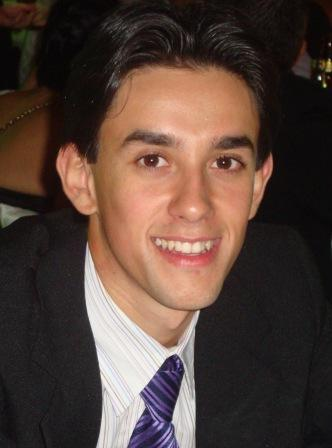
\includegraphics[width=0.15\textwidth]{figuras/foto-jean}
\end{wrapfigure}
O segundo número da nossa \textit{Newsletter} inaugura a seção de divulgação de novas publicações em pedometria. Todos podem contribuir enviando informações básicas sobre novas publicações, sejam elas nacionais ou internacionais. Basta enviar a contribuição ao editor responsável pela seção de novas puvlicações em pedometria, Jean Michel Moura-Bueno, pelo endereço de e-mail \email{bueno.jean1@gmail.com}.\\
As contribuições deverão ser sucintas, com tamanho inferior ao de um resumo geralmente apresentado em artigos científicos. Como estas contribuições servirão como propagandas de novos trabalhos publicados, é recomendado apresentar apenas informações chave, destaques que realmente chamam a atenção do leitor. Uma bom exemplo para ser seguido são os \emph{highlights} usados nos artigos da Elsevier: \emph{Os ``highlights'' são um pequeno conjunto de pontos que transmitem os resultados principais e fornecem aos leitores uma visão textual rápida do artigo}. Os resumos originais não serão publicados na \textit{Newsletter} por tal prática envolver questões de direitos dos autores e editoras das publicações originais.\\
Também é importante apresentar a forma de citação recomendada pelos autores, bem como o endereço da publicação na internet. Caso a publicação possua alguma figura interessante e autoexplicativa, a mesma deve ser enviada juntamente com o texto descritivo para a \textit{Newsletter}.
\section{Exemplo}
Abaixo há um exemplo utilizando uma publicação recente. Primeiro, é mostrado o resumo do artigo publicado no periódico científico e, em seguida, o formato recomendado para publicação na seção de novas publicações em pedometria da nossa \textit{Newsletter}.
\subsection{Título da publicação}
Building predictive models of soil particle-size distribution
\subsection{Citação}
A. Samuel-Rosa, R.S.D. Dalmolin, P. Miguel (2013) Building predictive models of soil particle-size distribution. {\em Revista Brasileira de Ciência do Solo} 37:422-430.
\subsection{Resumo original - não será publicado}
É possível construir modelos preditivos (MPs) da distribuição do tamanho de partículas do solo (DTP) em uma região que possua geologia complexa e uma superfície geomórfica jovem e instável? O principal objetivo deste trabalho foi responder a essa questão. Um conjunto de 339 amostras de solo de uma pequena bacia hidrográfica de encosta do sul do Brasil foi usado para construir MPs da DTP na camada superficial do solo. Modelos de regressão linear múltiplos foram construídos com atributos de terreno (elevação, declividade, área de captação, índice de convergência, índice de umidade topográfica). Os MPs explicaram mais da metade da variância dos dados. Esse desempenho é semelhante (se não melhor) ao da abordagem tradicional de mapeamento de solos. Para algumas frações de tamanho, o desempenho dos MPs pode chegar a 70\%. As maiores incertezas ocorrem nas áreas de maior complexidade geológica. Assim, melhorias significativas nas predições somente poderão ser alcançadas se dados geológicos acurados forem 
disponibilizados. Enquanto isso, MPs construídos a partir de atributos de terreno são eficientes em estimar a DTP de solos de regiões com geologia complexa.
\subsection{Resumo para a \textit{Newsletter}}
É possível construir modelos preditivos da distribuição do tamanho de partículas numa região com geologia complexa (arenitos e basaltos com arenito \emph{intertrap}) e superfície geomórfica jovem e instável? Esta é a pergunta que nos fez desenvolver este estudo em uma pequena bacia hidrográfica no RS. Com um conjunto de $n=339$ observações e alguns atributos de terreno, construímos modelos lineares para predizer a distribuição do tamanho de partículas na camada superficial do solo, tratados como dados composicionais. Os resultados sugerem que o desempenho dos modelos pode ser inferior, similar ou superior ao método tradicional de mapeamento do solo. As maiores incertezas estão conectadas às áreas onde as informações geológicas são mais pobres. Destacamos que a qualidade dos mapas geológicos deve ser melhorada se predições superiores forem demandadas.
\begin{footnotesize}
\begin{thebibliography}{99}
\bibitem[Samuel-Rosa et~al. (2013) Samuel-Rosa, Dalmolin, Miguel]{Samuel-RosaEtAl:2013} 
A. Samuel-Rosa, R.S.D. Dalmolin, P. Miguel (2013)
\newblock Building predictive models of soil particle-size distribution.
\newblock {\em Revista Brasileira de Ciência do Solo} 37:422-430. [\url{http://dx.doi.org/10.1590/S0100-06832013000200013}]
\end{thebibliography}
\end{footnotesize}
\address{Jean Michel Moura-Bueno\\
  Universidade Federal de Santa Maria\\
  \email{bueno.jean1@gmail.com}}
%%% Local Variables: 
%%% mode: latex
%%% TeX-master: documento-principal.tex
%%% End: 
\end{article}

\begin{article}
   \title{Eventos}
\maketitle


\section{INTERGEO}
\subsection{Istambul, Turquia, 28-29/4/2014}
O congresso é organizado pela German Society of Geodesy, Geoinformation and Land Management (DVW). 
Maiores informações podem ser encontradas no endereço \url{http://www.intergeo-eurasia.net/en/index.html}.


\section{Conferência e Feira de Geomática e Soluções Geoespaciais}
\subsection{São Paulo, Brasil, 7-9/5/2014}
O evento é organizado por MundoGEO.
Maiores informações podem ser encontradas no endereço \url{http://mundogeoconnect.com/2014/}.


\section{ISRIC'S Spring School 2014}
\subsection{Wageningen, Holanda, 12-16/5/2014}
O evento é organizado pelo International Soil Reference and Information Centre - ISRIC. Serão abordados temas relacionados ao Mapeamento Digital de Solos (MDS) e uso de softwares para análise de dados de solos.
Maiores informações podem ser encontradas no endereço \url{http://www.isric.org/content/isrics-spring-school-2014}.


\section{20th Word Congress of Soil Science}
\subsection{Jeju, Korea, 8-13/06/2014}
O congresso é organizado pela International Union of Soil Sciences (IUSS). 
Maiores informações podem ser encontradas no endereço \url{http://www.20wcss.org/}.


\section{12th International Conference of Precision Agriculture}
\subsection{Sacramento, Califórnia (USA), 20-23/07/2014}
O congresso é organizado pela Sociedade Internacional de Agricultura de Precisão.
Maiores informações podem ser encontradas no endereço \url{https://www.ispag.org/ICPA/}.


\section{XX Congresso Latinoamericano de la Ciencia Del Suelo}
\subsection{Cusco, Perú, 9-15/11/2014}
O evento é organizado pela Sociedade Latinoamericana de Ciência do Solo (SLCS).
Maiores informações podem ser encontradas no endereço \url{http://www.xxcongresolatinoamericanodesuelosperu.org/programa.php}.


\section{6th Global Workshop on Digital Soil Mapping}
\subsection{Nanjing, China, 11-14/11/2014}
O evento é  organizado pelo Instituto de Ciência do Solo da Academia Chinesa de Ciências. O prazo para submissão de trabalhos é 31/07/2014.
Maiores inforamçoes podem ser encontradas no endereço \url{http://dsm2014.csp.escience.cn/}.


\address{Jean Michel Moura-Bueno\\
    Universidade Federal de Santa Maria\\
    \email{bueno.jean1@gmail.com}}
\end{article}

\begin{article}
   \title{Instruções aos autores}
\maketitle
\newcommand{\SBCS}{\href{http://www.sbcs.org.br/}{SBCS}}
\newcommand{\Nature}{\href{http://www.nature.com/nature/authors/gta/}{Nature}}
\newcommand{\Science}{\href{http://www.sciencemag.org/about/authors}{Science}}
\newcommand{\CreativeCommons}{\href{http://creativecommons.org/licenses/by-sa/2.0/}{CC-BY-SA}}
\newcommand{\Kile}{\href{http://kile.sourceforge.net/}{Kile}}
\newcommand{\MiKTeX}{\href{http://miktex.org/}{MiKTeX}}
\newcommand{\aquiLaTeX}{\href{https://docs.google.com/document/d/1F3IXzWNCeUrwKeFxA4iHS3aw1nforK1IqB126xbawvA/edit?usp=sharing}{aqui}}
\newcommand{\aquiWord}{\href{https://docs.google.com/document/d/1pyK03RBDPhOMrTVfvj9NcEfjGWeswqYbYDqEKq83drQ/edit?usp=sharing}{aqui}}
\newcommand{\Geoderma}{\href{http://www.elsevier.com/author-schemas/latex-instructions}{Geoderma}}
\newcommand{\EJSS}{\href{http://onlinelibrary.wiley.com/journal/10.1111/\%28ISSN\%291365-2389/homepage/ForAuthors.html}{European Journal of Soil Science}}

\subsection{Escopo e política}

\pedometria{} é a \textit{Newsletter} (boletim técnico-científico) da Comissão de Pedometria da Sociedade Brasileira de Ciência do Solo (\SBCS). Assim sendo, dedica-se à publicação de artigos relacionados à aplicação de métodos matemáticos e estatísticos para o estudo da gênese e distribuição dos solos, o que abrange desde discussões conceituais até a aplicação prática de sensores e modelos. Especificamente, os seguintes tópicos costumam ser cobertos:

\begin{itemize}
 \item explicitação de conceitos pedométricos;
 \item entrevista com pedometrista;
 \item opinião sobre tema pedométrico relevante;
 \item descrição de equipamentos e sensores remotos;
 \item descrição de softwares e suas funcionalidades;
 \item eventos técnico-científicos;
 \item expressão artística em pedometria;
 \item novas publicações científicas em pedometria.
\end{itemize}

Os artigos submetidos para publicação em \pedometria{} NÃO DEVEM ser formais como aqueles geralmente submetidos para revistas científicas tradicionais da área de pedometria. DEVE-SE usar linguagem CLARA e INFORMAL, preferencialmente na VOZ ATIVA. O uso da voz ativa é uma recomendação para publicação em ambas as revistas \Nature{} e \Science:

\begin{description}
 \item \textit{Nature} ``Nature journals like authors to write in the active voice (`we performed the experiment...') as experience has shown that readers find concepts and results to be conveyed more clearly if written directly.''
 \item \textit{Science} ``Use active voice when suitable, particularly when necessary for correct syntax (e.g., `To address this possibility, we constructed a lZap library ...,' not `To address this possibility, a lZap library was constructed...').''
\end{description}

Conceitos pedométricos devem ser introduzidos com SENSIBILIDADE, tendo em mente que os leitores podem os desconhecer e/ou não possuir base conceitual suficiente para compreendê-los em uma única leitura. A estrutura do artigo deve ser concebida da mesma maneira que o fazemos para contar uma história a um amigo ou familiar, a fim de cativar o leitor e envolvê-lo no emocionante universo da pedometria. Caso a comissão editorial entenda que a compreensão do texto exija aprofundado conhecimento prévio do leitor, os autores serão solicitados a torná-lo mais simples e amigável.

O escopo e política de \pedometria{} coloca-a como veículo de divulgação e desmistificação da pedometria no Brasil. Trata-se de uma publicação com três edições anuais que permite aos pesquisadores brasileiros divulgar suas pesquisas pedométricas e, sobretudo, conhecerem uns aos outros. Isso é importante porque, assim como a própria pedometria, a maioria dos pedometristas também são bastante jovens, muitos dos quais ainda estão desenvolvendo seus estudos de mestrado e/ou doutorado. Por este motivo, \pedometria{} é distribuída gratuitamente via Internet, estando registrada sob a licença Creative Commons Atribuição-Compartilha Igual 3.0 Não Adaptada (\CreativeCommons).\\
\\
\begin{figure}[h!]
 \centering
 
\includegraphics[width=0.8\textwidth]{figuras/cc-by-sa}
 \caption{Licença Creative Commons Atribuição-Compartilha Igual 3.0 Não Adaptada.}
\end{figure}

\subsection{Estrutura do artigo}

A estrutura do artigo é inteiramente definida pelo(s) autor(es). Sugere-se que sejam utilizadas subdivisões em até dois níveis de profundidade (seções e subseções), não necessariamente definidas como em artigos científicos tradicionais. Os artigos podem ter, além do título, um subtítulo. Resumo e palavras-chave não são utilizados.

\subsubsection{Figuras e tabelas}

Figuras e tabelas são recomendadas, sendo uma foto do(s) autor(es) obrigatória. Figuras devem ser preparadas no formato PNG, com resolução mínima de 300 dpi.

\subsubsection{Referências bibliográficas}

Referências bibliográficas não são mandatórias, sobretudo no caso de artigos apresentando a opinião do autor sobre um tema pedométrico. Caso citações sejam feitas ao longo do texto, a lista de referências deve ser organizada na ordem em que as citações são feitas no texto. Importante notar que o estilo de citação numérica sobrescrita da \textit{Nature} é utilizado.

A lista de referências bibliográficas deve conter até cinquenta itens. O conteúdo da lista de referências deve ser econômico, incluindo apenas informações fundamentais para a sua identificação. Artigos, trabalhos em anais de eventos ou em coleções, e trabalhos publicados em veículos periódicos similares, devem ser formatados da seguinte maneira:

\vspace{0.5cm}
\noindent{A.B. McBratney, M.L. Mendonça-Santos, B. Minasny (2003) On digital soil mapping. \textit{Geoderma}, 117:3-52. \doi{10.1016/S0016-7061(03)00223-4}}
\vspace{0.5cm}

\noindent{onde \textit{link} refere-se ao endereço na Internet onde o referido documento pode ser encontrado. No caso de artigos científicos recomenda-se utilizar o Digital Object Identifier (\href{http://www.doi.org/}{DOI}). Livros, teses, dissertações, relatórios e outros meios de publicação não periódicos devem ser formatados da seguinte maneira:}

\vspace{0.5cm}
\noindent{H. Jenny (1994) \textit{Factors of soil formation - a system of quantitative pedology}. Toronto: Dover Publications.}
\vspace{0.5cm}

\noindent{Caso as publicações não periódicas estejam disponíveis na Internet, um link deve ser adicionado assim como para as publicações periódicas.}

\subsection{Preparo do artigo}

Os artigos podem ser preparados utilizando processadores de texto tradicionais, como por exemplo o MS Office Word (*.doc) e o LibreOffice Writer (*.odt), ou a linguagem de marcação \LaTeX() (*.tex). Preferência deve ser dada ao formato \LaTeX() sempre que possível a fim de facilitar o trabalho da equipe editorial. Documentos no formato PDF não são aceitos.

\subsubsection{Word ou Writer}

Um modelo para preparo do artigo usando processadores de texto tradicionais pode ser acessado clicando \aquiWord.

\subsubsection{\LaTeX}

\href{http://pt.wikipedia.org/wiki/Latex}{\LaTeX} é uma \href{http://pt.wikipedia.org/wiki/Linguagem_de_marca\%C3\%A7\%C3\%A3o}{linguagem de marcação} amplamente utilizada para a produção de textos matemáticos e científicos devido à sua alta qualidade tipográfica. Utilizar uma linguagem de marcação para elaboração de textos constitui no uso de comandos escritos para definir a formatação do documento, ao contrário dos editores tradicionais que oferecem abas e caixas de diálogo para clicar e definir parâmetros de formatação. Na prática, ao produzir um texto em \LaTeX, o autor não vê o produto final formatado na tela do computador imediatamente, mas apenas o texto e os comandos de formatação. O objetivo é distanciar o autor o máximo possível da apresentação visual do artigo, ou seja, ao invés de trabalhar com ideias visuais, o autor é encorajado a trabalhar com conceitos lógicos independentes da apresentação final do artigo. Além disso, linguagens de marcação como o \LaTeX{} permitem agilizar a confecção do documento final (PDF) e reproduzir o conteúdo em outros formatos para apresentação em meio digital como o html. Atualmente, importantes revistas científicas da área de pedometria adotam o \LaTeX{} para a confecção de seus artigos, como por exemplo \Geoderma{} e \EJSS.

Apesar de diferente dos processadores de texto tradicionais, usar \LaTeX{} é bastante fácil, sendo necessário apenas compreender a sua lógica de funcionamento. Para isso é bom dar uma olhada no \href{http://www.stdout.org/~winston/latex/}{Manual Rápido \LaTeX{}} para conhecer alguns comandos básicos. O preparo dos artigos usando \LaTeX{} pode ser feito usando softwares como Bloco de Notas, WordPad, e Gedit. Entretanto, é mais aconselhado usar um software específico para a edição de documentos em \LaTeX, como o \Kile{} e o \MiKTeX. Tais softwares auxiliam a inserção dos comandos necessários para a formatação do texto sem a necessidade de memorizá-los.

Um modelo para preparo do artigo usando \LaTeX{} pode ser acessado clicando \aquiLaTeX.

\subsection{Submissão}

Qualquer pessoa pode submeter um artigo para publicação em \pedometria{} sem qualquer custo. Quando o artigo estiver pronto, adicione todos os arquivos utilizados (inclusive as figuras originais) à uma pasta comprimida e envie para a comissão editorial usando o endereço de e-mail \email{pedometria.news@gmail.com}.

\subsection{Comissão editorial}

Alessandro Samuel-Rosa\\
\textit{ISRIC - World Soil Information}\\
\textit{Wageningen University and Research Center}\\
\email{alessandro.rosa@wur.nl}\\
\\
André Geraldo de Lima Moraes\\
\textit{Curso de Pós-Graduação em Agronomia-Ciência do Solo}\\
\textit{Universidade Federal Rural do Rio de Janeiro}\\
\email{andrehmuz@hotmail.com}\\
\\
Diego Silva Siqueira\\
\textit{Grupo de Pesquisa Caracterização do Solo para fins de Manejo Específico}\\
\textit{Universidade Estadual Paulista - Campus Jaboticabal}\\
\email{diego\_silvasiqueira@yahoo.com.br}\\
\\
Jean Michel Moura-Bueno\\
\textit{Programa de Pós-Graduação em Ciência do Solo}\\
\textit{Universidade Federal de Santa Maria}\\
\email{bueno.jean1@gmail.com}

\subsection{Observação}

Iniciamos tratativas com a Sociedade Brasileira de Ciência do Solo para que toda a sua documentação e números publicados de \pedometria{} fiquem hospedados no \textit{website} \url{http://www.sbcs.org.br}. Infelizmente a Sociedade  Brasileira de Ciência do Solo não possui infraestrutura disponível para que isso seja possível. Enquanto isso, \pedometria{} fica temporariamente hospedada no \textit{website} \url{https://sites.google.com/site/pedometria/}, impedindo a obtenção de ISSN.

\subsection{Agradecimento}

Gostaríamos de agradecer o conselho editorial do \href{http://grass.osgeo.org/newsletter/}{GRASS News} do projeto GRASS pois, sem a sua contribuição com os arquivos *.tex e *.sty do GRASS News, \pedometria{} teria levado muito mais tempo para atingir o nível atual.
%%% Local Variables: 
%%% mode: latex
%%% TeX-master: 4rd-edition.tex
%%% End:
\end{article}

\end{document}

%%% Local Variables: 
%%% mode: latex
%%% TeX-master: documento-principal.tex
%%% End: 
